\documentclass[usenatbib]{mn2e}

\usepackage{amsmath}
\usepackage{graphicx}
\usepackage{epstopdf}
\usepackage{multicol}

\title{Microlensing as a possible probe of event-horizon structure in quasars}
\author[Tomozeiu et al]{Mihai Tomozeiu\thanks{mihai@physik.uzh.ch},$^{1,2}$ 
Irshad Mohammed,$^{1,2,3}$ 
Manuel Rabold,$^{1,2}$
Prasenjit Saha,$^{1,2}$  
\newauthor
and Joachim Wambsganss$^{1,4}$\\
$^1${Physik-Institut, University of Zurich, Winterthurerstrasse 190,
  8057 Zurich, Switzerland} \\
$^2${Institute for Computational Science, University of Zurich,
  Winterthurerstrasse 190, 8057 Zurich, Switzerland} \\
$^3${Theoretical Astrophysics Group, Fermi National Accelerator Laboratory, Batavia, IL 60510, USA}\\
$^4${Zentrum f\"ur Astronomie der Universit\"at Heidelberg,
  M\"onchhofstrasse 12--14, 69120 Heidelberg, Germany}
}

\begin{document}

\maketitle

\begin{abstract}

In quasars which are lensed by galaxies, the point-like images sometimes show sharp and uncorrelated brightness 
variations (microlensing). These brightness changes are associated with the innermost region of the quasar passing 
through a complicated pattern of caustics produced by the stars in the lensing galaxy. In this paper, we study 
whether the universal properties of optical caustics could enable extraction of shape information about the central 
engine of quasars. We present a toy model with a crescent-shaped source crossing a fold caustic. The silhouette 
of a black hole over an accretion disk tends to produce roughly crescent sources. When a crescent-shaped source 
crosses a fold caustic, the resulting light curve is noticeably different from the case of a circular luminosity 
profile or Gaussian source. With good enough monitoring data, the crescent parameters, apart from one degeneracy, 
can be recovered.

\end{abstract}


\begin{keywords}
Supermassive black holes, microlensing, quasars.
\end{keywords}

\section{The General Picture }

Active galactic nuclei (AGN) are thought to be powered by the accretion of
matter from the proximal environment into a supermassive black hole.
The radiation emitted excites the surrounding medium which becomes
detectable as narrow line regions, broad line regions and optical
continuum.  In the direction perpendicular to the accretion disc,
where the medium is more transparent, the outflowing material tends to be
collimated to jets.  If the orientation is such that the observer's
view of the central region is not blocked by the accretion disc or by
a jet, a quasar is seen \citep[e.g.,][]{1984RvMP...56..255B}.  While
the basic mechanism \citep[originating in the work
  of][]{1964ApJ...140..796S,1964SPhD....9..246Z,1969Natur.223..690L}
is not in doubt, the central engines, near the event horizons of the
black holes, remain to be probed.

Modestly active galactic nucleii are present in the Galactic centre
and in M87.  In these two cases, the central engines ($<0.1\rm\,mas$
on the sky) are close to being resolved through very long baseline
interferometry, which shows preliminary indications of the
jet-launching structures
\citep{2008JPhCS.131a2055D,2012Sci...338..355D,2016ApJ...820...90F}.
Current data do not deliver images but require fitting to predefined
models for the images.  A whole range of models have been applied,
starting from simple geometric models to more complex physical models
\citep{2008Natur.455...78D,2011ApJ...738...38B,2009ApJ...706..497M,2010ApJ...717.1092D}.
The more complicated models nonetheless tend to predict a crescent
shaped silhouette of the black hole.  This motivated
\cite{2013MNRAS.434..765K} to use a simple geometric crescent model to
fit the available sub-mm interferometric data. They argued that the
crescent is nothing but the silhouette of the event horizon.
The great majority of quasars, however, lie at redshifts beyond 2
\citep{2014A&A...563A..54P} and their central engines would be orders
of magnitude smaller on the sky. The direct observations of the black
hole silhouettes of quasars are far beyond foreseeable
instrumentation.

In the present paper, we consider a possible indirect method, related
to \cite{1999ApJ...524...49A} and \cite{2015ApJ...814L..26M}, 
through which gravitational
microlensing could probe the black hole shadow and its proximal quasar
environment.

%Gravitational microlensing of quasars, reviewed in
%Section~\ref{sec:microlensing} below, refers to sharp changes in the
%observed brightness of quasars that have been lensed by an intervening
%galaxies, without any changes in the intrinsic luminosity.  

Gravitational microlensing of quasars, reviewed in
Section~\ref{sec:microlensing} below, is a phenomenon seen in quasars
that have been multiply imaged by galaxies.  Individual images in a
multiple-image system can undergo sharp and seemingly random
brightness changes.  This can occur, even for constant intrinic
luminosity, as a consequence of two things: the very small size of the
central engine, and granularity of the mass distribution of a lensing
galaxy due to stars.  The latter means that the local magnification is
not a smooth function of source position. It contains a complicated
network of singular curves, known as caustics.
Figure~\ref{fig:magnification_map} shows part of a magnification map
with a few caustics.  The lensed brightness would be given by placing
the source on such a magnification map and integrating the surface
brightness weighted by the magnification.  Most astrophysical sources
straddle several caustics, and hence, their net brightness varies
smoothly with location.  The central engine of quasars, however, is
smaller than the typical spacing between caustics.  As a result, the
lensed brightness undergoes sudden changes as a quasar crosses a
caustic.  Quasar microlensing is observable at optical
wavelengths \citep[e.g.,][]{2012A&A...544A..62S} and in
X-rays \citep[e.g.,][]{2016arXiv160207601N}.  In principle, it exists
at all wavelengths \citep[and has been argued for at cm wavelengths
  by][]{2000A&A...358..793K} but will be washed out if the light is
from larger regions than the central engine of the quasar.  The effect
thus supplies an upper limit on the size of the central engine
\citep[e.g.,][]{2015ApJ...814L..26M} and can be used to study the mass
distribution of stars in the lensing galaxy as well
\citep[e.g.,][]{2012ApJ...744..111P}.  Microlensing caustics have an
additional remarkable feature: though they can be very complicated,
they have some universal properties well-known from catastrophe
theory.  In particular, very close to the simplest caustics (known as
folds), the magnification is approximately constant on one side and
$\propto1/\sqrt p$ where $p$ is the transverse distance of the source
from the caustic.  This property will be exploited later.

In Section~\ref{sec:source-models} we introduce three source profiles
which are used in our subsequent models and simulations: a
constant-brightness disc, a circular Gaussian, and the crescent source
introduced by \cite{2013MNRAS.434..765K}.  The latter is simply a
constant-brightness disc with a smaller, non-concentric disc cut out
of it.  We also derive the half-light radius for a crescent.  The
half-light radius can characterise the source size for all three types
of source.

Section~\ref{sec:fold-crossing} shows the light curves that result
when each of the model sources crosses an ideal fold.  This would
apply in Figure~\ref{fig:magnification_map} to sources along the path
AB or BC, for sources small enough that the curvature of the caustics
is negligible.  With this assumption one can imagine the caustic as an
infinite wall to be crossed by the source as presented in
Figure~\ref{fig:infinite_fold}.  The source brightness distribution
parallel to the caustic naturally makes no difference to the
observable brightness; each source can be replaced by an effective
one-dimensional source profile, by flattening the source so it becomes
perpendicular to the caustic.  In principle, the effective
one-dimensional brightness profile could be recovered from the light
curve by deconvolution.  \cite{1999ApJ...524...49A} modelled this
profile as the result of a circular accretion disc seen through the
spacetime around a Kerr black hole, and \cite{2012MNRAS.423..676A}
have applied the idea to observed light curves to infer properties of
quasar accretion discs.  A similar idea appears in
\cite{2013ApJ...769..131C}.  In this work, we take a simpler but
arguably more robust approach: we study features in the light curves
characteristic of a crescent-like source which in turn would indicate
a black-hole silhouette.  Figure~\ref{fig:char_points} shows the
qualitative features: there is a period during which the dark cutout
disc is crossing the caustic, and before and after there are periods
when the only the bright parts of the crescent are in transit across
the caustic.  The details depend on the orientation of the crescent,
but basically the dark disc causes a rising light curve to plateau or
dip.  These features are still present, albeit faintly, if the simple
crescent is replaced by a source based on an accretion-disc simulation
of a black-hole environment (Figure~\ref{fig:M87_plots}).

In Section~\ref{sec:numerics} we carry out source fitting to
lightcurves, with both noise and systematic errors are present.  We
generate a mock lightcurve by taking a crescent source across the path
CB in Figure~\ref{fig:magnification_map}, and then adding noise.  The
path simulates crossing a clean but not ideal fold.  We then fit this
lightcurve to templates from both crescent and circular-Gaussian
sources along the paths AB as well as CB.  That is, the templates from
a similar but not identical caustic are also used, thus deliberately
generating a systematic error.  Despite this systematic error, a
crescent source fits the data, while a Gaussian source is rejected
from the $\chi^2$ value.

Finally in Section~\ref{sec:discussion} we discuss in more depth the
implications of the results presented in the previously mentioned
sections.  One of the most interesting implications is the possibility
of estimating the black hole mass from the reconstructed
parameters. This further requires good approximations of the relative
transversal velocity between the quasar and the lens. Proper
constraints can be set with independent observations of the stellar
structure that contain the gravitational lens.

The thorough study of the possibility to reconstruct the quasar's
structural parameters from light-curves containing multiple
microlensing events represents the target of future work. This will
most probably require the use of powerful statistical tools. Another
path for future work is the designing of an observation regime best
suited for acquiring the necessary microlensed light-curve.


\section{Microlensing}\label{sec:microlensing}

We start by introducing in a succinct manner the gravitational lensing
theory that is relevant for microlensing in general and for the scope
of the present paper in particular.  More detailed presentation of the
theory can be found in several references, such as
\cite{2001stgl.book.....P}.

\subsection{Magnification}

The gravitational lens equation
\begin{equation}
\vec\beta = \vec\theta - \vec\alpha(\vec\theta)
\label{eqn:lens}
\end{equation}
relates the apparent sky position $\vec\theta$ of a light source to
its true but unobservable sky position $\vec\beta$ through the bending
angle $\vec\alpha$.  The latter is an integral 
\begin{equation}
\vec\alpha = (1+z_{_L})\frac{D_S-D_L}{D_SD_L} \frac{4G}{c^2}
\int \Sigma(\vec\theta')
\frac{\vec\theta-\vec\theta'}{|\vec\theta-\vec\theta'|^2}\,
d^2\vec\theta'
\label{eqn:alpha}
\end{equation}
depending on the projected density $\Sigma(\vec\theta)$ (kg/steradian)
of the lens, the lens redshift $z_{_L}$ and the comoving distances
$D_L$ and $D_S$ to the lens and source.  The derivative of the
apparent position with respect to the source position
\begin{equation}
M(\vec\theta) =
\left(\frac{\partial\beta}{\partial\theta}\right)^{-1}
\label{eqn:magnif-matrix}
\end{equation}
is known as the magnification matrix, and its determinant
\begin{equation}
\mu(\vec\theta) = \det|M(\vec\theta)|
\end{equation}
is the brightness amplification of an image of a point source.  In
other words, the source will brighten or dim according to whether
$\mu(\vec\theta)$ is more or less than unity.  If there are multiple
images at distinct but not observationally resolved $\vec\theta_i$ from
the same $\vec\beta$, a total brightness amplification
of

\begin{equation} \mu_{\rm total} = \sum_{i} \mu(\vec\theta_i)
\end{equation}
applies. It is possible for the magnification to become formally
infinite, as a result of an eigenvalue of the magnification matrix
(\ref{eqn:magnif-matrix}) becoming infinite.  This generically happens
on curves on the $\vec\theta$ plane, known as {\em critical curves}.
Mapping a critical curve to the source plane, through the lens
equation (\ref{eqn:lens}), to the source plane $\vec\beta$ gives the
so-called caustics.  Caustics can appear in the optical system, not just
during gravitational lensing.  For a point source, caustics are singularities
of the magnification; for finite-size sources caustics correspond to
high and sharply changing magnification.

Caustics are important in all forms of lensing with multiple images,
but they have a special significance for lens quasars, first pointed
out by \cite{1979Natur.282..561C}.  The granularity of the mass
distribution $\Sigma(\vec\theta)$ due to individual stars produces a
caustic network on the scale of $\sqrt{GM_\odot D_L/c^2}$ or $10^{-6}
\sqrt{M/M_\odot}\rm\,arcsec$ for typical lens and source redshift
\citep{2001PASA...18..207W}.  Extended sources wash out this
micro-caustic structure, but the optical-continuum and X-ray sources
of quasars are even smaller.

\begin{figure}
\centering
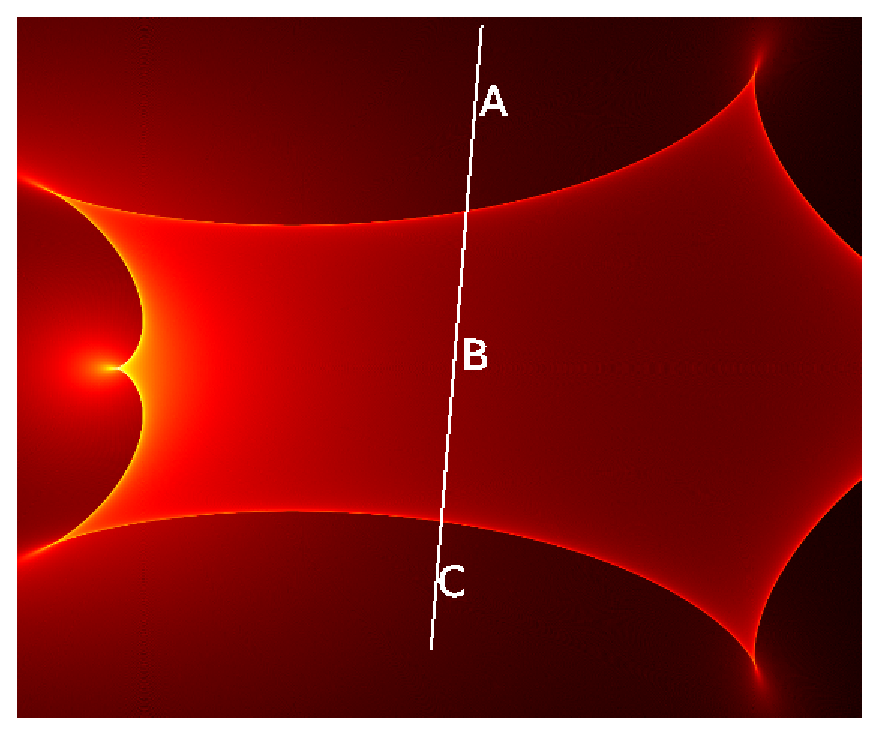
\includegraphics[width=0.9\hsize]{figures/IRIS567_path.eps}
\caption{\label{fig:magnification_map} Magnification map used later in
  this paper (Section~\ref{sec:numerics}). The white line marks the
  trajectory of the center of the sources for which the lightcurves
  presented in figures \ref{fig:cc_forward}, \ref{fig:cc_backward} and \ref{fig:gc_forward} are generated.  Note that this represents an
  atypically simple region of any realistic magnification map.}
\end{figure}


\subsection{Magnification near a fold caustic}

A simple example of a caustic network is shown in
Figure~\ref{fig:magnification_map}.  There are two general categories
of caustics in gravitational lensing, cusps and fold, and examples of
both kinds can be seen in this figure.  Magnification near a caustic
has universal properties, independent of the system and has been
extensively studied
\citep{1986ApJ...310..568B,1992A&A...260....1S,2002ApJ...574..970G,2002ApJ...580..468G}.
In particular, at distance $p$ from a fold caustic
\begin {equation}
 \mu(p) = \mu_0 + C_0 \frac{1}{\sqrt{p}} \Theta(p).
\end {equation}
Here the magnification of a point source near a caustic is equal to
the sum of the magnification due to other reasons $\mu_0$ 
(such as zero point magnification and the effect of other weaker and 
distant lenses), assumed to
be locally constant, and a decrease with the square root of the
distance from the fold. The latter term becomes activated only after
the source enters the region interior to the caustic curves when the
values of the step function $\Theta(p)$ become unity. The
proportionality constant $C_0$ depends on the local conditions in the
vicinity of the caustic.

A source of arbitrary shape can be described by a two-dimensional brightness function $S_{2D}(p - p_s, q - q_s)$ defined for a coordinate system $p,q$ where $p_s, q_s$ denote the coordinates of the center of a source.

\begin{figure}
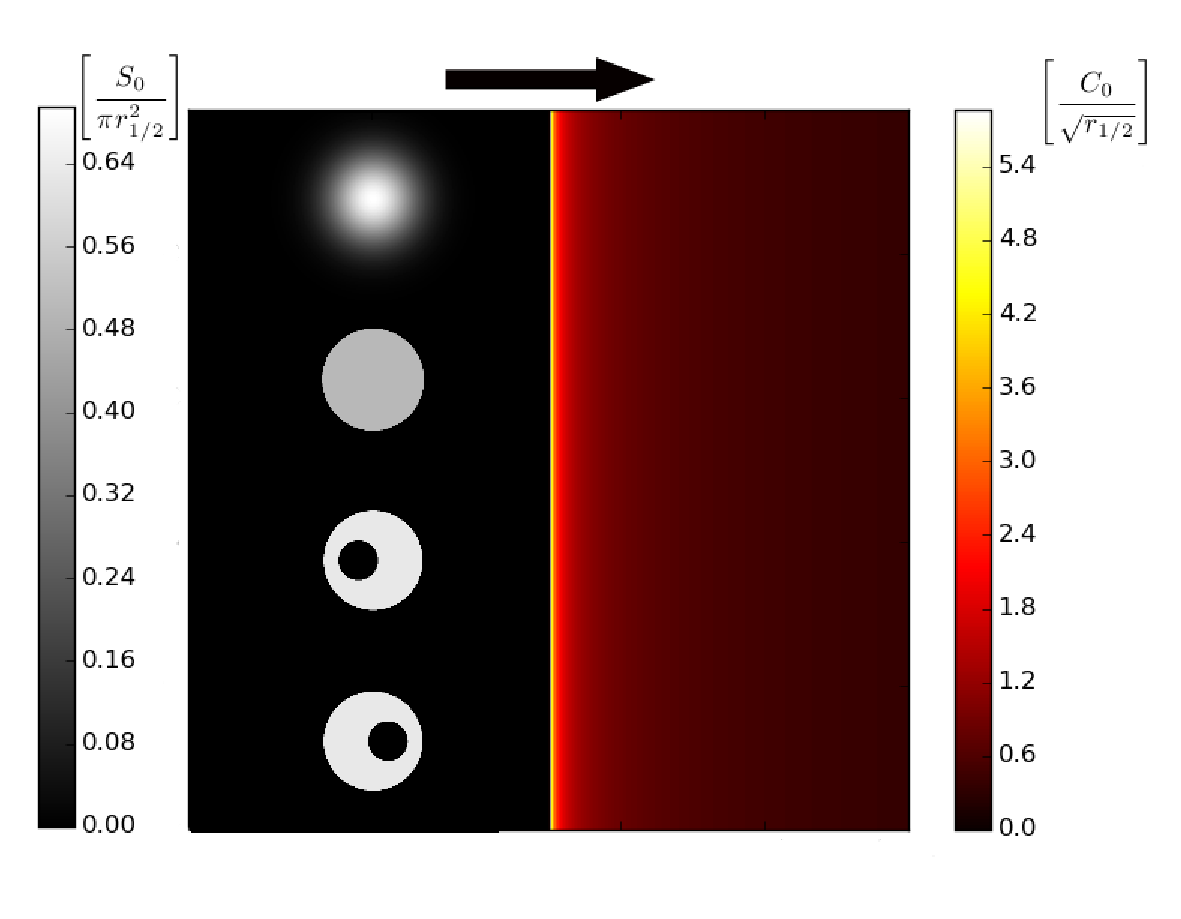
\includegraphics[width = .49\textwidth]{figures/infinite_fold_ar.eps}
\caption{\label{fig:infinite_fold} Source profiles for Gaussian, disk,
  crescents (right) and magnification map for an infinite fold
  (left). Objects have the same $S_{0}$ and $r_{1/2}$. The black arrow marks the direction of motion of the
sources relative to the caustic.}
\end{figure}

For a microlensing event the lightcurve can be written for an
arbitrary source shape as:
\begin{equation}
 F(t) = \int_{-\infty}^\infty \int_{-\infty}^\infty S_{2D}(p-p_s(t), q-q_s(t)) \mu_t(p) \mathrm{d}q \mathrm{d}p.
 \label{eqn:ft2d}
\end{equation}
In order to build the previous equation we have considered that the
time dependency of the flux $F$ is given only by the motion of the
source with respect to a fixed caustic. Therefore the only time
dependent quantities in the right hand side of the equation are the
coordinates of the center of the source $p_s(t),q_s(t)$.

Due to the choice of coordinate system the amplification factor 
has no dependence on the $q$ coordinate. The previous equation can be rewritten as:

\begin{equation}
 F(t) 
= \int_{-\infty}^\infty  \mu_t(p) S_{1D}\left(p-p_s(t)\right) \mathrm{d}p,
\label{eqn:ft}
\end{equation}
\\
where we have defined the one dimensional flux function as:
\begin{equation}
 S_{1D}(p-p_s(t)) = \int_{-\infty}^\infty S_{2D}(p-p_s(t), q-q_s(t)) \mathrm{d}q
\end{equation}

This representation is a valid approximation only when the apparent size of the source is much smaller than the corresponding Einstein angle of the lens. In this context 
all the information about the source shape and brightness that can be contained in the lightcurve is exhaustively given by the 1D flux function.
In other words, if two sources with different $S_{2D}$ have the same $S_{1D}$ they cannot be distinguished by studying their lightcurves.
 
 
\section{Models for extended sources}\label{sec:source-models}

In the present study we analyse three types of sources with different surface brightness: 
\begin{enumerate}
 \renewcommand{\theenumi}{(\arabic{enumi})}
  \item a rotationally symmetric source with a bivariate Gaussian surface brightness distribution,
  \item a disk source with constant surface brightness distribution,
  \item a crescent shaped source with constant surface brightness distribution.
\end{enumerate}
The first two sources are the typical choices used in the literature to describe the luminous parts of a quasar. 
The third one is a recently proposed variant \citep{2013MNRAS.434..765K}.




\subsection{Rotationally symmetric source with a bivariate Gaussian surface brightness distribution}\label{subsec:gaussian}

A symmetric 2D Gaussian can be described mathematically as:

\begin{equation}
 S_{2D}^G(p-p_s, q-q_s) = \frac{S_0^G}{2 \pi \sigma^2} e^{-\frac{(p-p_s)^2}{2 \sigma^2}} e^{-\frac{(q-q_s)^2}{2 \sigma^2}}.
\end{equation}
\\
The corresponding 1D brightness is:

\begin{equation}
 S_{1D}^G(p-p_s) = \frac{S_0^G}{\sqrt{2 \pi} \sigma} e^{-\frac{(p-p_s)^2}{2 \sigma^2}}.
\end{equation}
\\
Other parameters of the model are the total flux $S_0^G$ and $\sigma$. 

Although such a definition for a source would have non-zero surface/linear brightness for any coordinate $p,q$, the amount of light received by a detector from outside a $3 \sigma$ disk centered at $p_s, q_s$ 
would be insignificant. For a Gaussian distributed surface brightness source the half-light radius is directly proportional to the parameter $\sigma$ according to the equation:
\begin{equation}
r_{1/2} = \sqrt{\ln4}\,\sigma.
\end{equation}

\subsection{Disk source with constant surface brightness distribution}

One can construct mathematically a disk source with constant surface brightness and radius $R$ using a stepfunction:
\begin{equation}
 S_{2D}^D(p-p_s, q-q_s) = \frac{S_0^D}{\pi R^2} \Theta \left( R^2 - \left( p-p_s \right)^2 - \left( q-q_s \right)^2 \right).
\end{equation}
By integrating over $q$ coordinate the linear brightness function is obtained:


\begin{equation}
 S_{1D}^D(p-p_s) = \frac{2 S_0^D}{\pi R}  \sqrt{1 - \frac{(p-p_s)^2}{R^2} }    \Theta \left( R^2 - \left( p-p_s \right)^2 \right).
\end{equation}
The half-light radius of a uniform disk source is $R/\sqrt{2}$.

\subsection{Crescent source with constant surface brightness distribution}\label{subsec:crescent}

The surface brightness distribution of a geometric crescent can be built 
by considering two disk sources of constant brightness. One larger disk 
will contribute positively to the total flux while one smaller disk 
that is interior to the large one will contribute negatively. This superposition can be written for 2D as:\\

\begin{equation}
 S_{2D}^C =  S_{2D}^{Dp} -  S_{2D}^{Dn}  
 \label{eqn:s2d}
\end{equation}
with\\

\begin{equation}
 S_{2D}^{Dp}(p-p_{sn}, q-q_{sn}) = \frac{S_0^{Dp}}{\pi R_p^2} \Theta \left( R_p^2 - \left( p-p_{sp} \right)^2 - \left( q-q_{sp} \right)^2 \right)
\end{equation}
\\
and
\begin{equation}
 S_{2D}^{Dn}(p-p_{sn}, q-q_{sn}) = \frac{S_0^{Dn}}{\pi R_n^2} \Theta \left( R_n^2 - \left( p-p_{sn} \right)^2 - \left( q-q_{sn} \right)^2 \right).
\end{equation}
The following notations were used: $R_p$ and $(p_{sp}, q_{sp})$ are
the radii and coordinate of the center for the larger positive disk, 
while $R_n$ $(p_{sn},q_{sn})$ correspond to the smaller negative disk. 
$S_0^{Dp},S_0^{Dn}$ represent the total flux of radiation received from the large and small disk. 
From this point forward we will not use the total flux from each source. Instead we will 
use the difference which in this case is the total flux from the crescent-shaped source $S_0^C$. \\
Equation \ref{eqn:s2d} can be written as:\\

\begin{align}
 S_{2D}^C &= \frac{S_0^C}{\pi \left(R_p^2-R_n^2 \right)} \left\{ \Theta \left[ R_p^2 - \left( p-p_{sp} \right)^2 - \left( q-q_{sp} \right)^2 \right] \right.\nonumber\\
 &\qquad \left. {} -  \Theta \left[ R_n^2 - \left( p-p_{sn} \right)^2 - \left( q-q_{sn} \right)^2 \right] \right\}.
\end{align}
\\
Analogously for the linear brightness function:

\begin{align}
 S_{1D}^C &= \frac{2 S_0^C}{\pi \left(R_p^2-R_n^2 \right)} \left\{ \sqrt{R_p^2 - (p-p_{sp})^2}  \Theta \left[ R_p^2 - \left( p-p_{sp} \right)^2 \right] \right.\nonumber\\
 &\qquad \left. {} - \sqrt{R_n^2 - (p-p_{sn})^2 } \Theta \left[ R_n^2 - \left( p-p_{sn} \right)^2 \right] \right\}.
\label{eqn:s1_d}
\end{align}


There are some constraints on the parameters used to define a crescent
in the previously presented manner that need to be stated. First, we
must impose the obvious $R_p \geq R_n$ relation. Secondly, the small disk
must always be interior to the large disk:
\begin{equation}
 R_p \ge R_n + \sqrt{\left(p_{sp} - p_{sn} \right)^2 + \left(q_{sp} - q_{sn} \right)^2}
\end{equation}
For the distances between the centers of the two disks we will use the same 
notations as the one found in the paper \citep{2013MNRAS.434..765K}, $a \equiv p_{sn} - p_{sp}$ and $b \equiv q_{sn} - q_{sp}$.

The half-light radius of any source is invariant under any rotational
transformation.  In the present case of a crescent source the
effective radius is dependent on the parameters $R_p$, $R_n$ and
$\sqrt{a^2+b^2}\equiv c $ exclusively. From symmetry considerations
the centroid of the source is collinear with the centers of the two
disks and it is situated at a distance $d_c$ from the center of the
bright disk. $d_c$ can be computed numerically with the use of a
variation of equation \ref{eqn:s1_d}:

\begin{equation}
\begin{aligned}
\frac{S_0^C}{2} & = \frac{2 S_0^C}{\pi \left(R_p^2-R_n^2 \right)} \int_{d_c}^{R_p} \bigg[ \sqrt{R_p^2 - p^2} \\ 
        & - \sqrt{R_p^2 - \left(p-c\right)^2} \Theta \left(R_p^2 - \left(p-c\right)^2 \right) \bigg] \mathrm{d}p. 
\end{aligned}
\end{equation}   

With the position of the centroid determined, the half-light radius
can be also be computed through a numerical integral:
 
\begin{equation}
\begin{aligned}
S_0^C &=  \frac{4S_0^C}{\pi \left(R_p^2-R_n^2 \right)} \int_{0}^{r_{1/2}} \left[ \Theta_2  - \Theta_1  \right] p \mathrm{d}p; \\
\Theta_1 &= \bigg[ \pi - \arccos \frac{R_p^2 + p^2 -d_c^2}{2 R_p p} \\
         & \phantom{= \bigg[ \pi} - \arccos \frac{R_p^2 - p^2 + d_c^2}{2 R_p d_c}
            \bigg] \Theta \left( p - R_p + d_c \right); \\
\Theta_2 &=  \pi - \arccos \frac{ p^2  + (c+d_c)^2 - R_n^2}
                                {2 p \left(c + d_c \right)} \\
         & \phantom{= \pi - } \Theta \left( p + R_n - d_c -c \right). 
\end{aligned}
\end{equation}

\begin{figure}
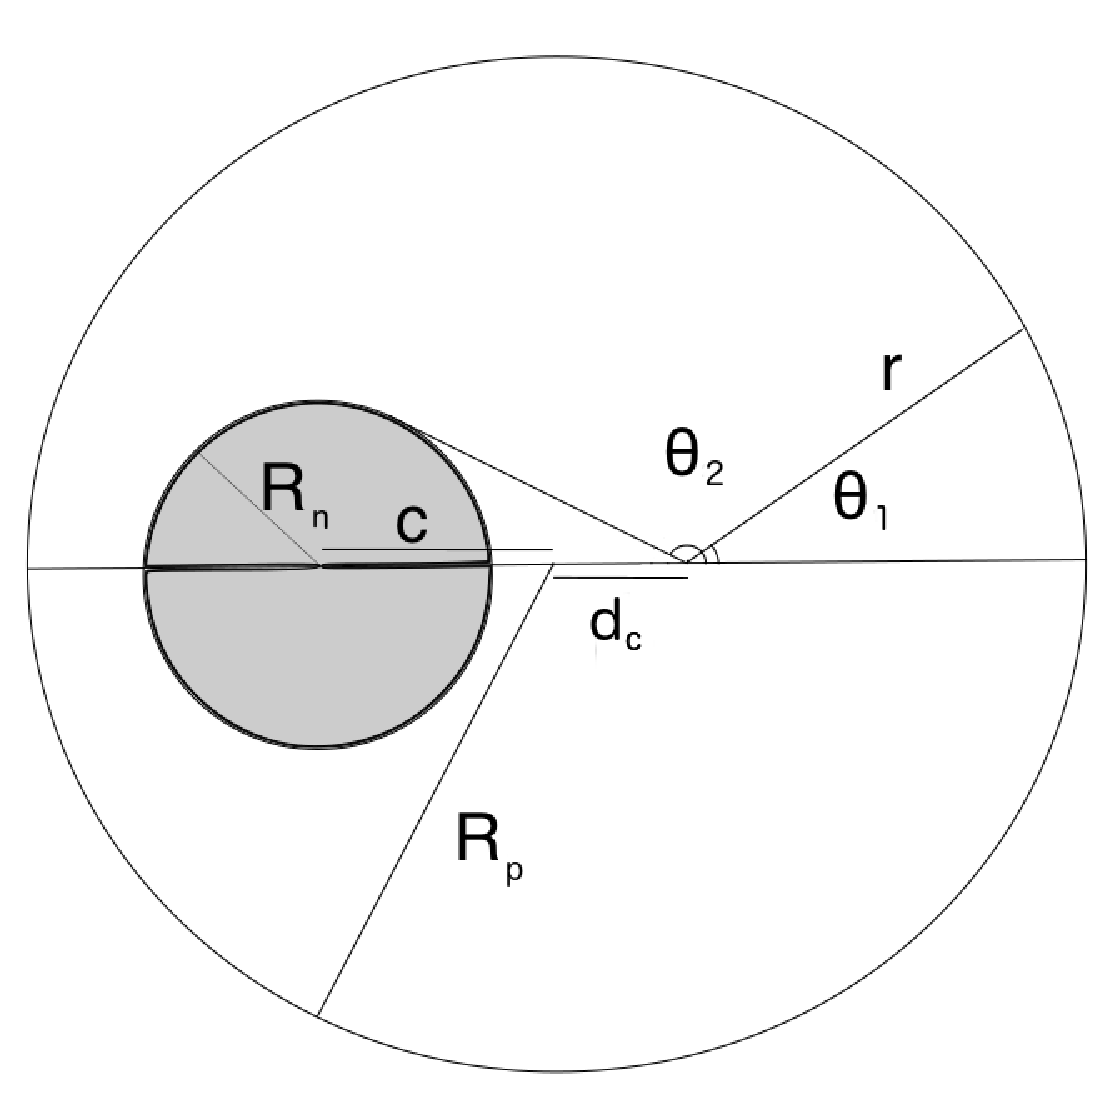
\includegraphics[width = .49\textwidth]{figures/figure_rhalf2.eps}
\caption{\label{fig:geom_crescent} Geometry of crescent sources: the source can be seen as a superposition
 of a smaller dark disk over and inside a larger brighter disk. $R_p$ and $R_n$ mark the radii of the 
bright and dark disk. $d_c$ and $c$ mark the distance from the center of the bright disk to the 
centroid and from the dark disk to the centroid.  }
\end{figure}


\section{Lightcurves of the extended sources during fold crossing}\label{sec:fold-crossing}

Using equation \ref{eqn:ft} and the one-dimensional flux function
presented in the previous section one can numerically compute the
lightcurves of the three extended sources for the simplified
infinite-wall-caustics model.

\subsection{Lightcurve of the Gaussian source}

The amount of light received by an observer from a source 
with a Gaussian distributed brightness with $\sigma$ and total flux $S_0^G$ in the absence of any gravitational lensing is:
\begin{equation}
 F^G(t) = \int_{-\infty}^\infty  \left( \mu_0 + \frac{C_0}{\sqrt{p}} \Theta \left( p \right) \right) \left( \frac{S_0^G}{\sqrt{2 \pi} \sigma} e^{-\frac{(p-p_s(t))^2}{2 \sigma^2}} \right) \mathrm{d}p.
\end{equation}
which can be simplified to:
\begin{equation}
 F^G(t) = \mu_0 S_0^G + \frac{C_0 S_0^G}{\sqrt{2\pi} \sigma} \int_{0}^\infty \frac{e^{-\frac{(p-p_s(t))^2}{2 \sigma^2}}}{\sqrt{p}} \mathrm{d}p.
\end{equation}


\begin{figure}
\centering
        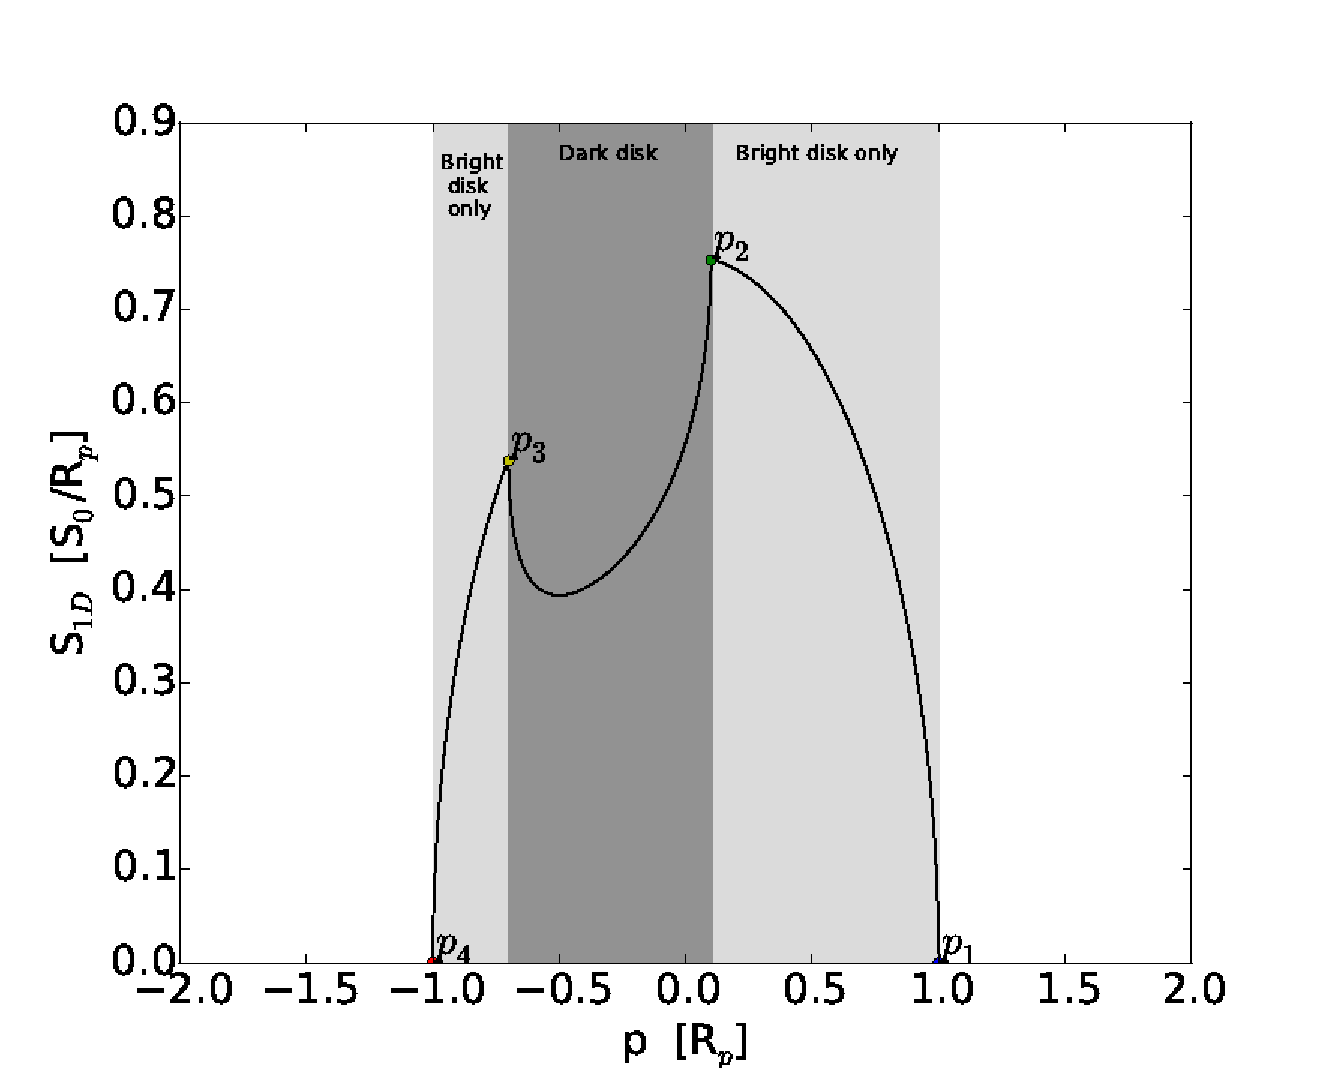
\includegraphics[width = 0.48\textwidth]{figures/ch_points.eps}
        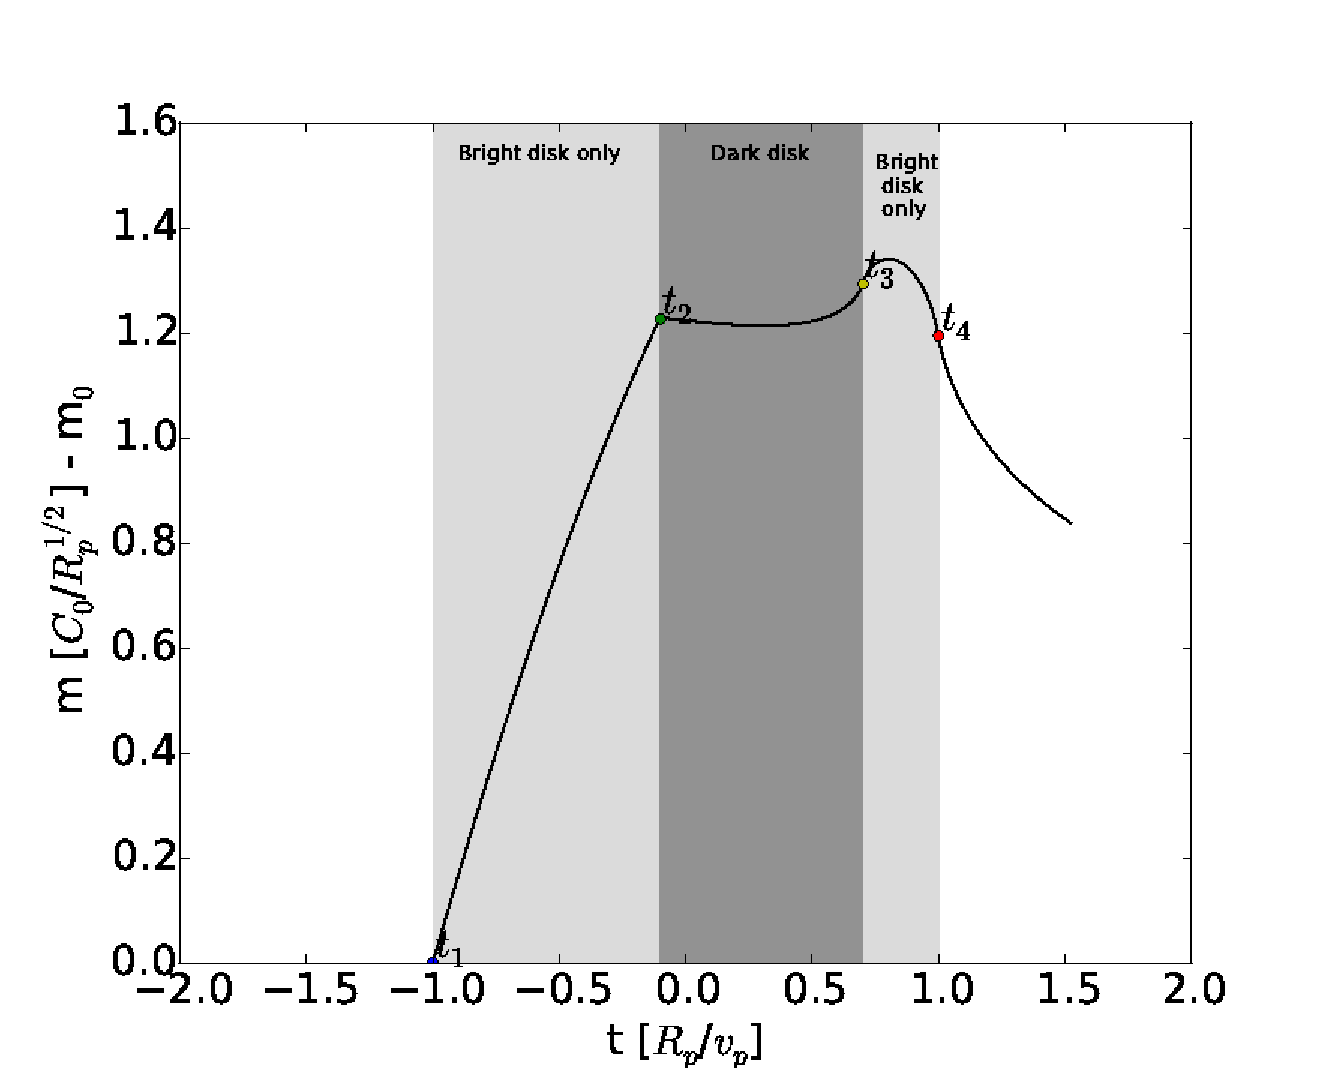
\includegraphics[width = 0.48\textwidth]{figures/ch_instances.eps}
\caption{\label{fig:char_points} The characteristic points and
  instances of a crescent source's one dimensional profile and
  microlensing lightcurve.  In the top panel a typical 1D profile of a
  crescent source is presented.  There are two light gray regions that
  mark the regions of the bright disk that are not overlapped by the
  dark disk. The dark gray band marks the region where the two disks
  overlap. The points $p_1$ and $p_4$ mark the start and end of the
  bright disk in the 1D representation. Analogously, $p_2$ and $p_3$
  mark the start and end of the dark disk.  The bottom panel
  represents the associated lightcurve with the points $t_i$ marking
  the moment when point $p_i$ overlaps with the caustic.  The gray
  shades are analogous to the ones in the top panel.  }
\end{figure}





\begin{figure}
\centering
    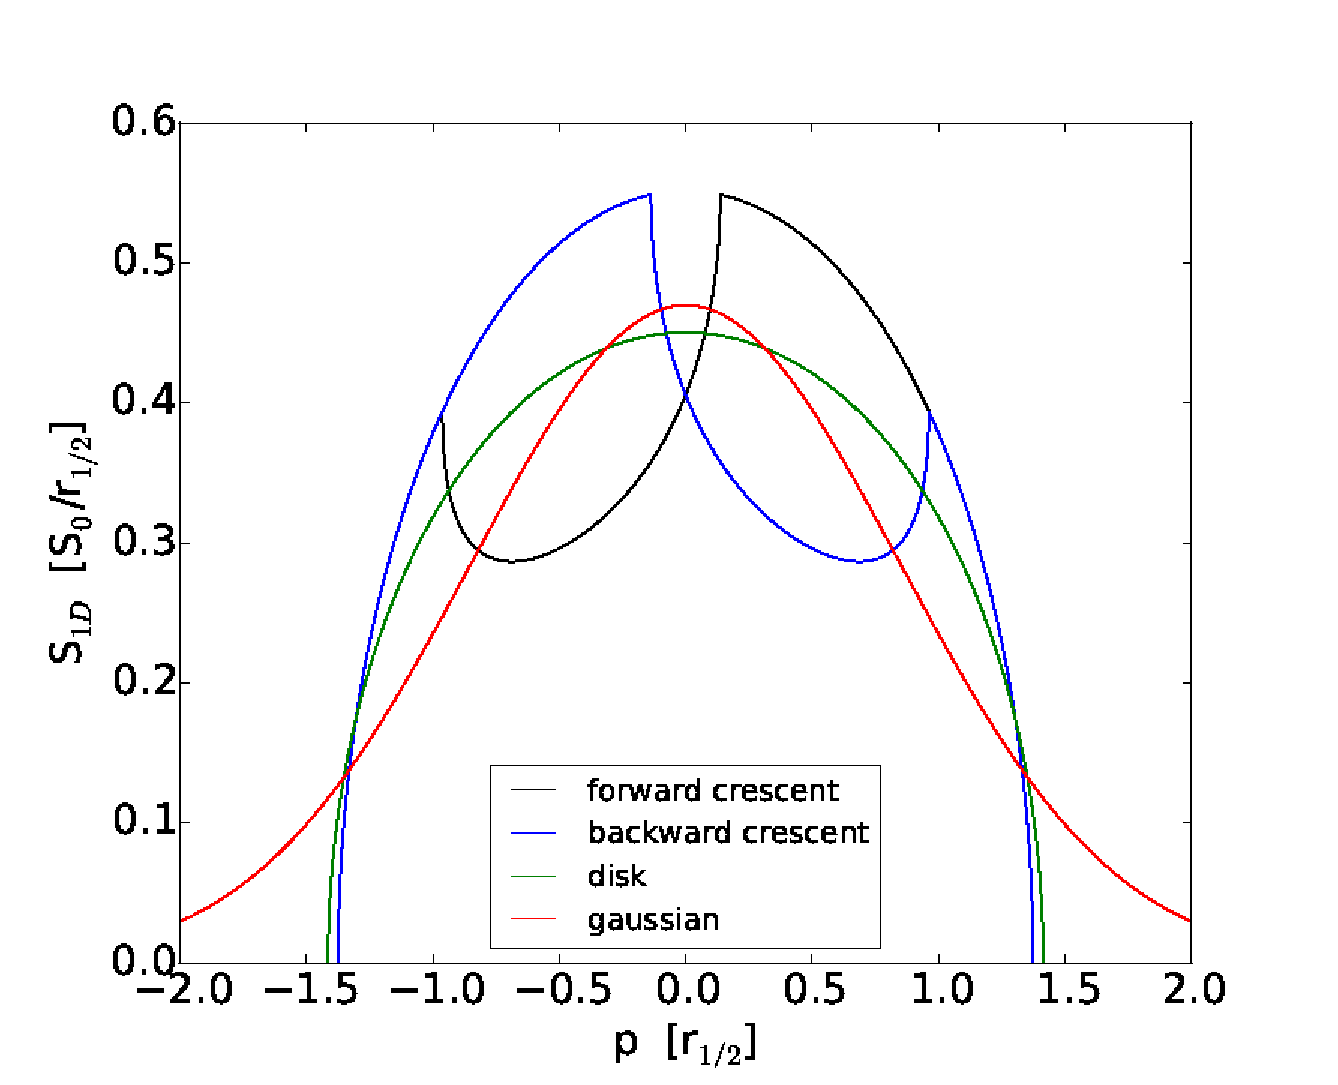
\includegraphics[width = 0.48\textwidth]{figures/S1D_all.eps}
    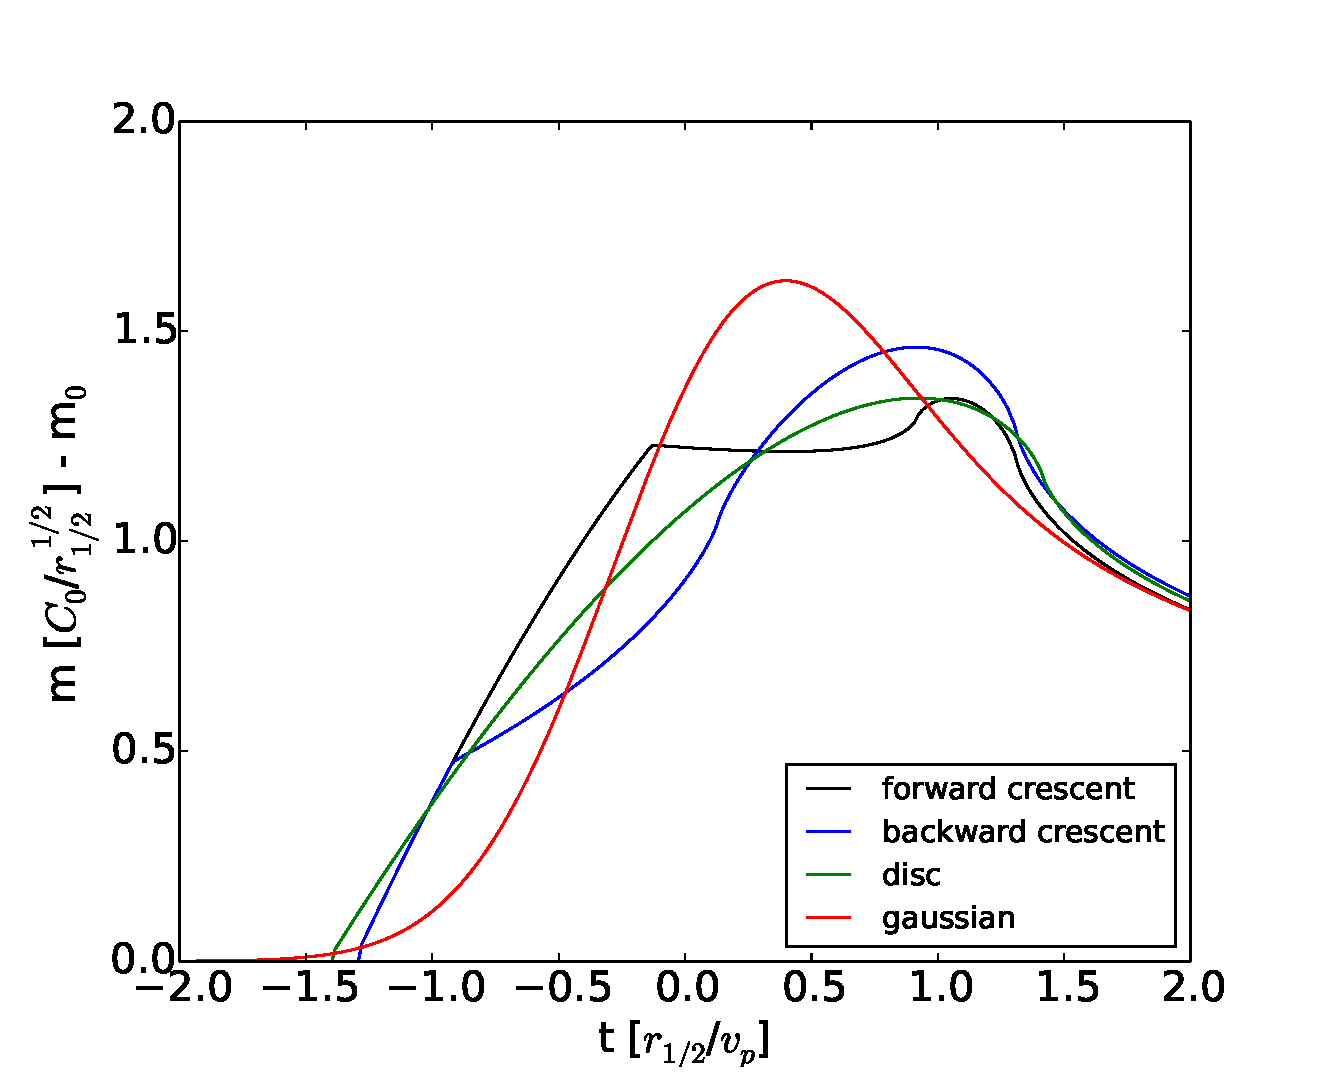
\includegraphics[width = 0.48\textwidth]{figures/4source_magnification.eps}
\caption{\label{fig:lightcurve_gauss} 1D profiles (top panel) and simulated lightcurves (bottom) of crescent, Gaussian and disk sources with identical total flux ($S_0$) and half-light radius($r_{1/2}$). Crescent source has $r_{1/2}$ = 0.72754 $R_p$, $R_n$ = 0.4 $R_p$, a = 0.3/-0.3 $R_p$. }
\end{figure}


\subsection{Lightcurve of the disk shaped source}

Analogous to the Gaussian shaped source, the disk source with uniform brightness, radius $R$ and 
unmagnified flux $S_0^D$ has a lightcurve described by the equation:

\begin{equation}
\begin{aligned}
 F^D(t) &= \int_{-\infty}^\infty  \left( \mu_0 + \frac{C_0}{\sqrt{p}} \Theta \left( p \right) \right) \\
    & \bigg[ \frac{2 S_0^D}{ \pi R} \sqrt{1 - \frac{\left( p-p_s(t) \right)^2}{R^2}}  \Theta \left(R^2 - \left(p-p_s(t) \right)^2 \right) \bigg] \mathrm{d}p.
\end{aligned}
\end{equation}
which is equivalent to:
\begin{equation}
 F^D(t) = \mu_0 S_0^D + \frac{2 C_0 S_0^D}{\pi R} \int_{max(0, p_s(t) - R)}^{max(0, p_s(t) + R)} \frac{1}{\sqrt{p}} \sqrt{1 - \frac{\left( p-p_s(t) \right)^2}{R^2}} \mathrm{d}p.
\end{equation}

\begin{figure}
\centering
    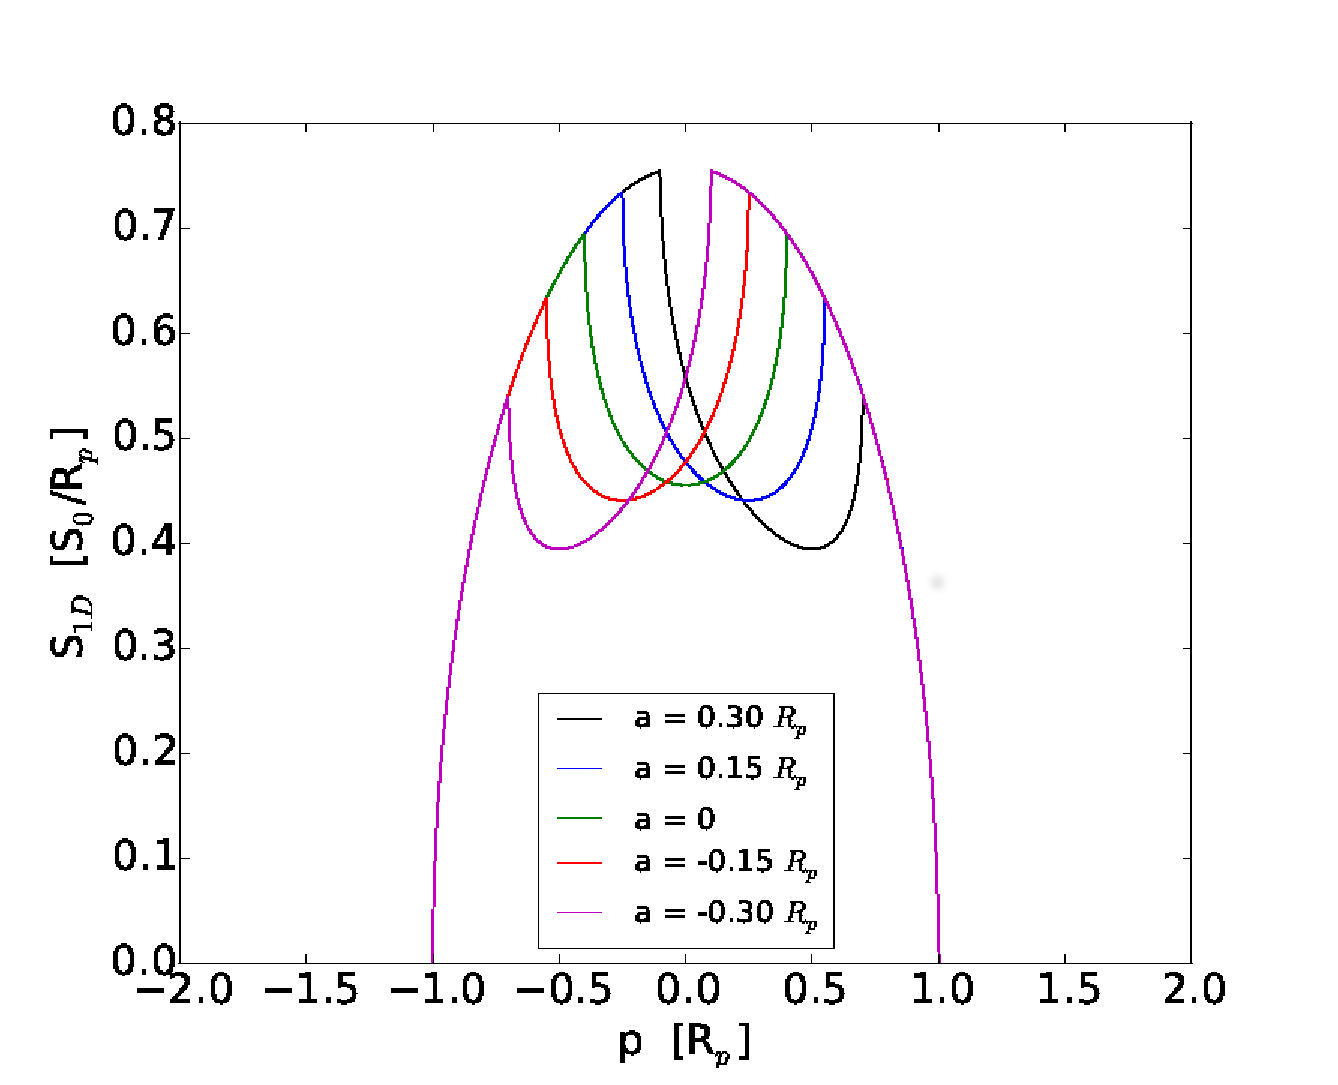
\includegraphics[width = 0.48\textwidth]{figures/S1D_var_a.eps}
    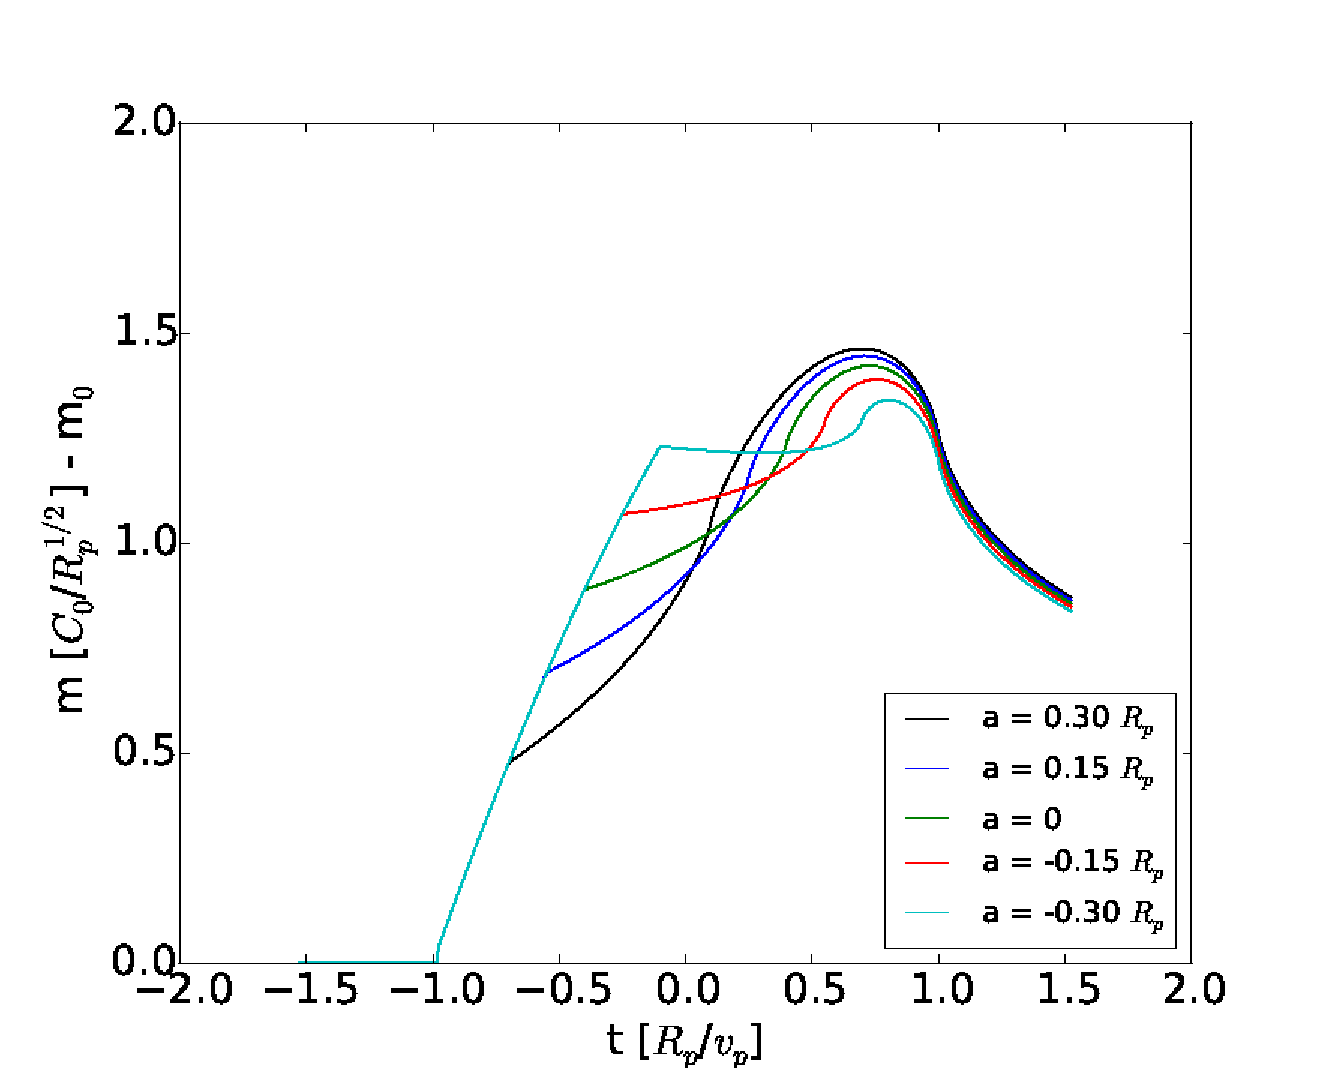
\includegraphics[width = 0.48\textwidth]{figures/4avar_magnification.eps}
\caption{\label{fig:a_var} 1D profiles (top panel) and simulated lightcurves 
(bottom) of crescent sources with identical $R_p$ and $R_n$ ($R_n$ = 0.4 $R_p$) and different disk centers displacement (a).}
\end{figure}


\subsection{Lightcurve of the crescent shaped source}

The lightcurve of a crescent shaped source with unamplified flux $S_0^C$, radii $R_p$, $R_n$ and center displacement $a(t)$ is:


\begin{equation}
\begin{aligned}
 F^c(t) &= \mu_0 S_0^C + C_0 \frac{2 S_0^C}{\pi \left( R_p^2 -R_n^2 \right) } \\
    &\bigg[ \int_{max(0, p_s(t) - R)}^{max(0, p_s(t) + R)} \sqrt{\frac{R_p^2 - \left( p-p_s(t) \right)^2 }{p}} \mathrm{d}p \\
    &  -  \int_{max(0, p_s(t) - a(t) - R)}^{max(0, p_s(t) -a(t) + R)} \sqrt{\frac{R_p^2 - \left( p-p_s(t) +a(t) \right)^2 }{p}} \mathrm{d}p  \bigg] .
\end{aligned}
\end{equation}


\begin{figure}
\centering
    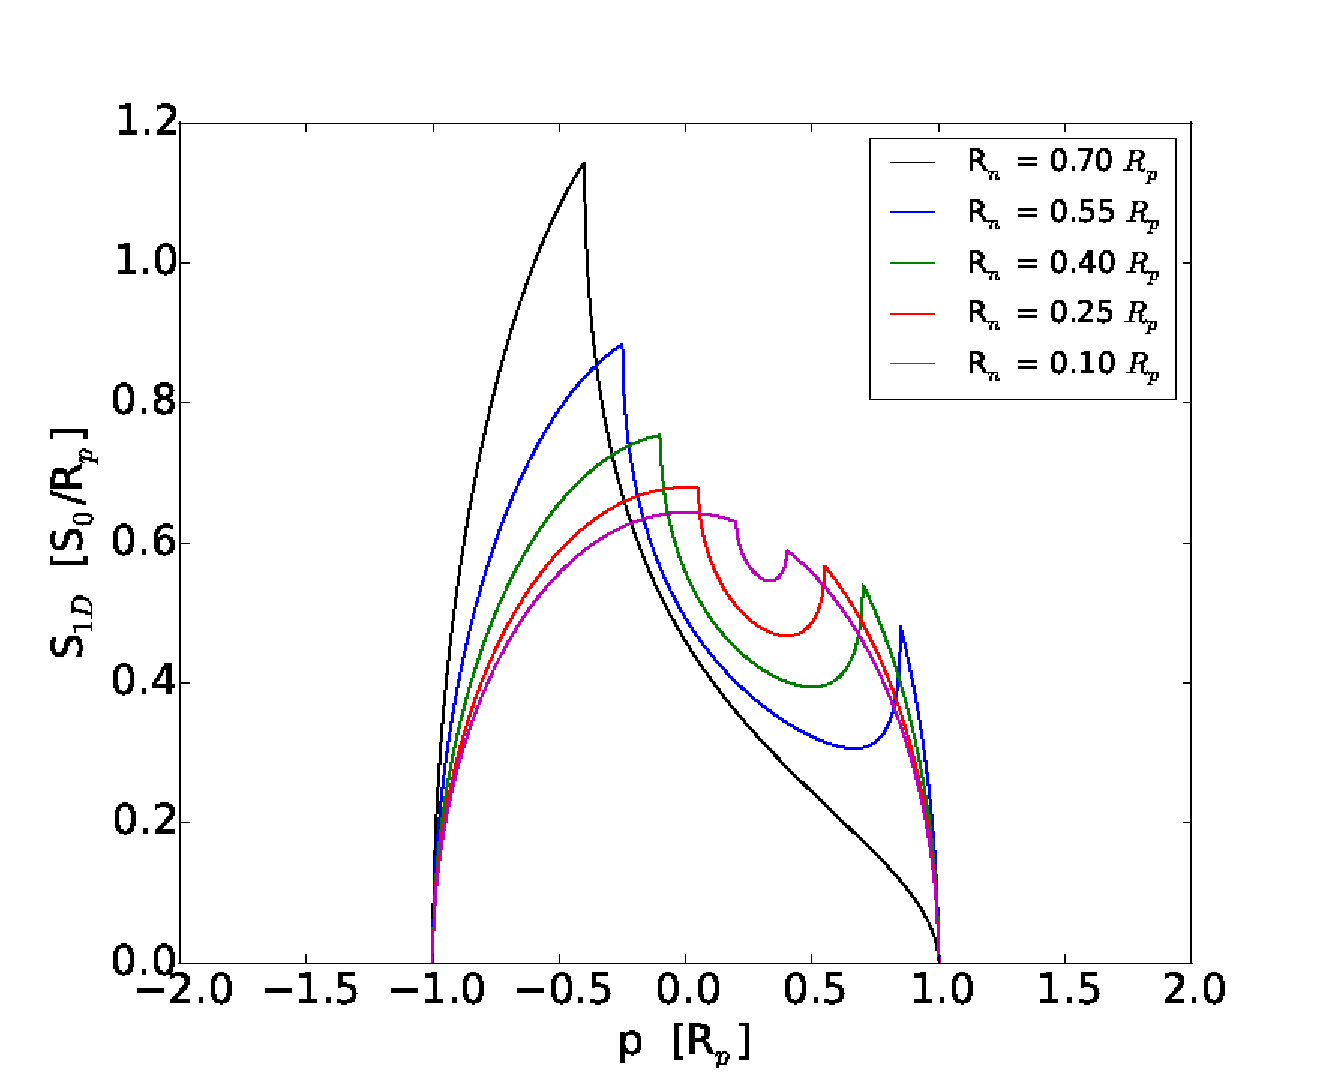
\includegraphics[width = 0.48\textwidth]{figures/S1D_var_rn_a_poz.eps}
    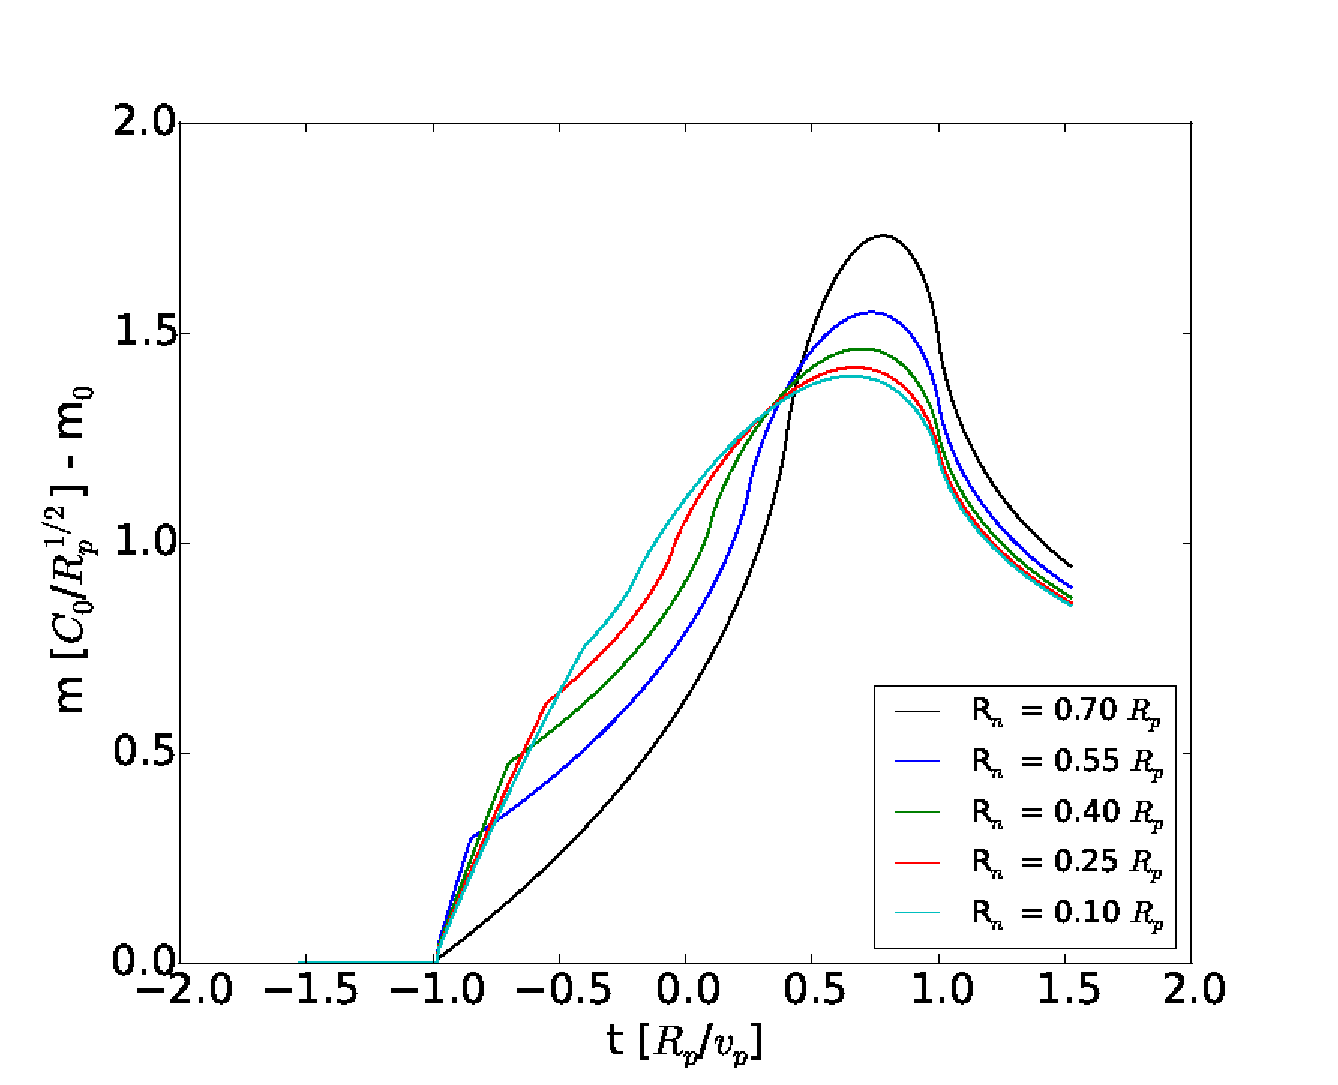
\includegraphics[width = 0.48\textwidth]{figures/5Rn_back_var_magnification.eps}
\caption{\label{fig:lightcurve_crescent_back} 1D profiles (top panel) and simulated lightcurves (bottom) of backwards crescent sources with identical $R_p$ and $a$ ($a$ = 0.3 $R_p$) and different dark disk radii ($R_n$).}
\end{figure}

The function $p_s(t)$ can be chosen to be equal to $v_p(t-t_0) + p_{s0}$ where $p_{s0}$ is the coordinate $p$ 
of the source at the initial time, and $v_p$ is the component of the velocity
along the $p$ axis. Such a model of the motion of the object in the source 
plane describes a linear motion with constant velocity. Furthermore, we reduce the complexity of the model by 
choosing the function $a$ to be constant in time.  

\begin{figure}
\centering
    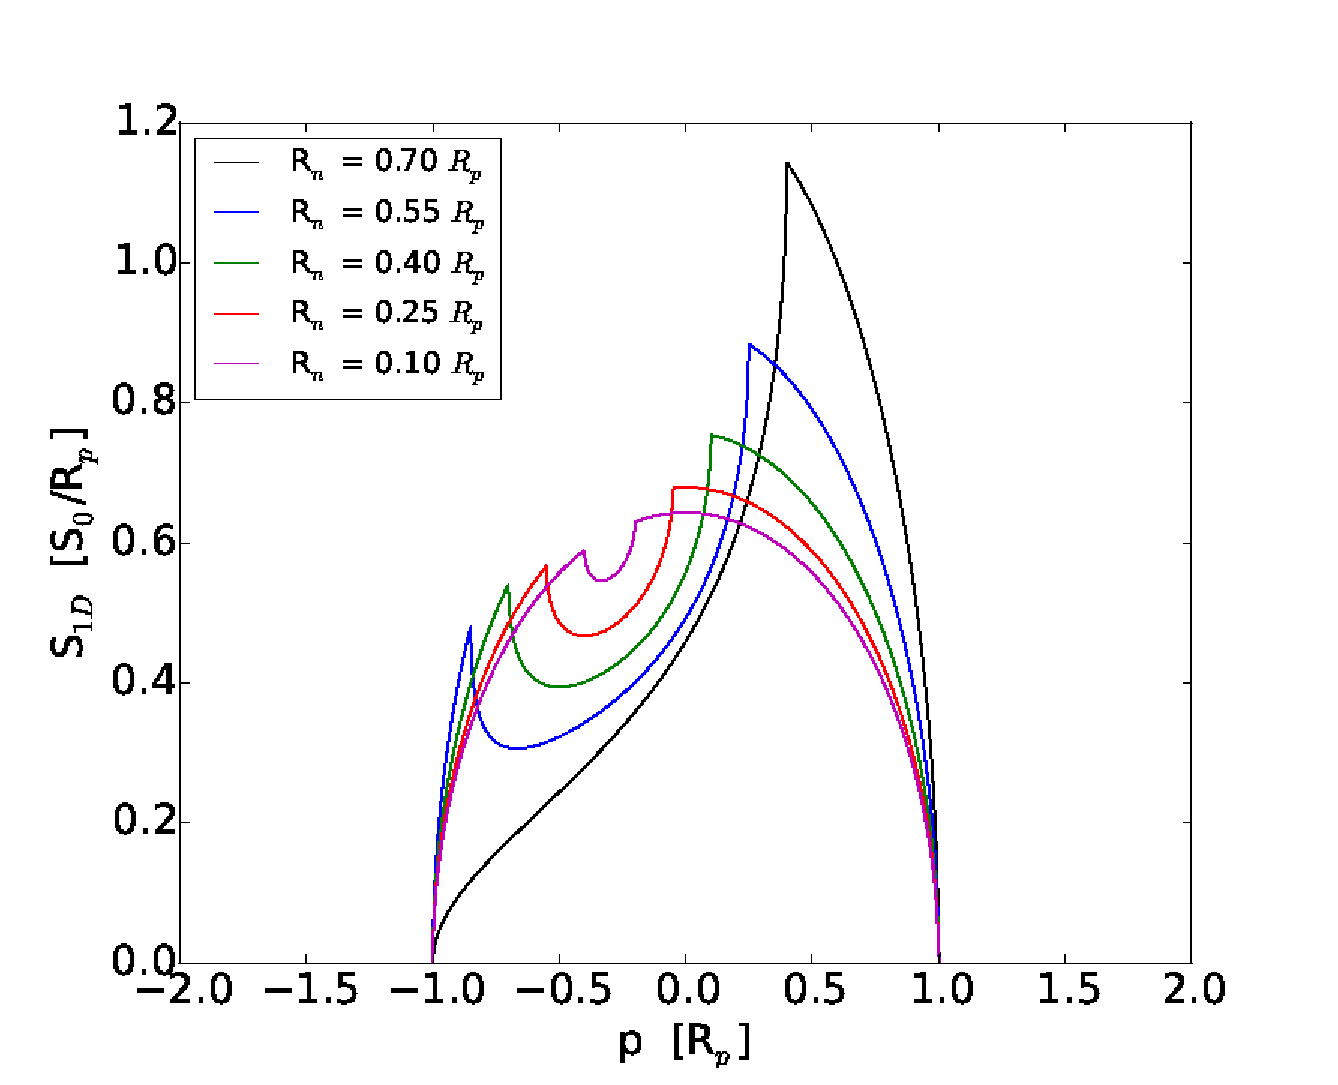
\includegraphics[width = 0.48\textwidth]{figures/S1D_var_rn_a_neg.eps}
    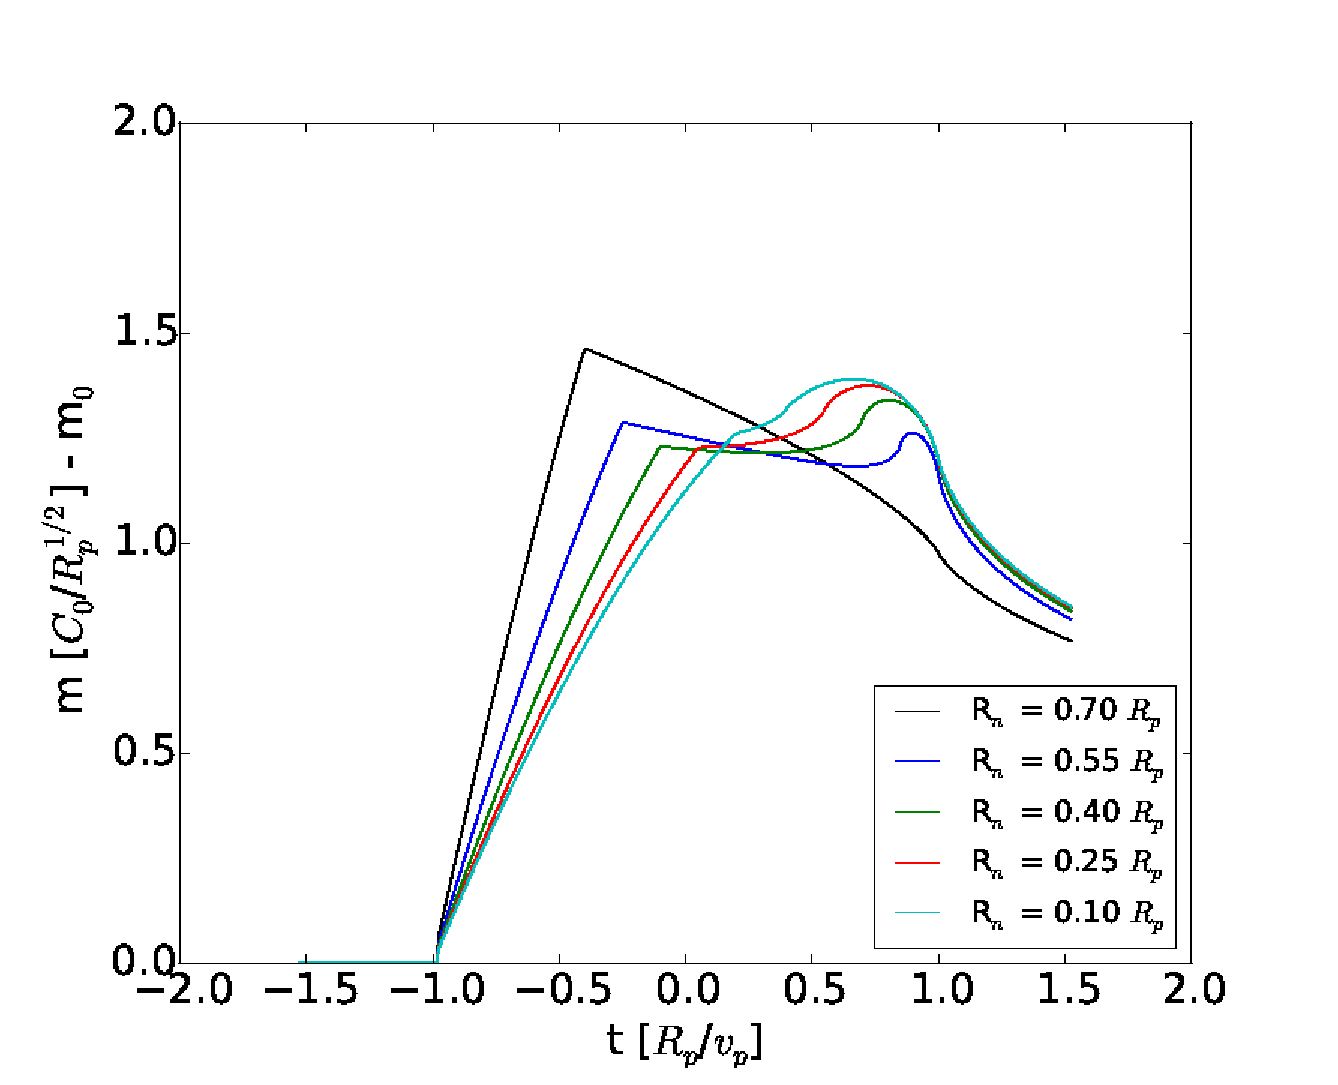
\includegraphics[width = 0.48\textwidth]{figures/5Rn_forw_var_magnification.eps}
\caption{\label{fig:lightcurve_crescent} 1D profiles (top panel) and simulated lightcurves (bottom) 
of forwards crescent sources with identical $R_p$ and $a$ ($a$ = - 0.3 $R_p$) and different dark disk radii ($R_n$). }
\end{figure}

In Figure \ref{fig:char_points} there are four characteristic points visible on the resulting one-dimensional 
light profile of the crescent shaped source. Two of the points, p1 and p4, mark the outer boundaries of the
 luminous disc component. The other two, p2 and p3, mark the boundaries of the dark disc component. 
Since $S_{1D}$ is a projection of $S_{2D}$ on a line perpendicular to the caustic, the following relation holds:
\begin{equation}
    p_2-p_1 = R_p -R_n - a.
\end{equation}
In addition there are two other obvious relations the characteristic points which are independent of the projection:
\begin{equation}
    p_4 -p_1 = 2 R_p,
\end{equation}

\begin{equation}
        p_3 -p_2 = 2 R_n.
\end{equation}
All four points mark the positions where the derivative $\frac{dS_{1D}}{dp}$ is discontinuous. The points can be used 
to define three regions: $p_1 - p_2$ where $S_{1D}$ is convex, $p_2 - p_3$ where $S_{1D}$ is concave, 
and $p_3 - p_4$ where $S_{1D}$ is convex again. \\

Due to the nature of the caustic and the monotonic behaviour of the magnification map on both sides of the caustic, the previously 
mentioned characteristic points are inherited by the microlensing lightcurve. The points on the temporal dimension 
$t_1, t_2, t_3$ and $t_4$ correspond to instances in time when the fold is aligned with $p_1, p_2, p_3$ and $p_4$, respectively. 
For a constant relative velocity $v_p$ between the source and the caustic there is a simple relation between the points $p_i$ and instances $t_i$:

\begin{equation}
    t_j - t_i = \frac{p_j - p_i}{v_p}.
\end{equation}

With the use of the previous four equations the following identities can be written:

\begin{equation}
    R_p = \frac{v_p \times  \left( t_4 -t_1 \right)}{2}, 
\end{equation}

\begin{equation}
        R_n = \frac{v_p \times \left( t_3 -t_2 \right)}{2}, 
\end{equation}

\begin{equation}
        a = \frac{v_p \times \left( t_4 +t_1 - t_3 - t_2 \right)}{2}. 
\end{equation}




Figure \ref{fig:lightcurve_gauss} reveals that the 
lightcurve of a crescent source has more
visible features than the other two light-curves corresponding to the
disc and Gaussian shape. There are three regions where $S_{1D}$ and by
inheritance, the lightcurve has distinguishable behaviour. The first
region that would be recorded on a lightcurve plot represents the
period of time when the bright disk begins to be overlapped by the
caustic and stops when just before the dark disk reaches the
caustic. During this period of time, the flux of light from the source
is increasingly magnified. The second period starts and ends with the
overlapping of the dark disc. As a boundary of the two regions, there
is a distinguishable point where the slope of the magnification is
drastically changed. This apparent discontinuity in the first
derivative of the magnification function is caused by the caustic
amplification of the sudden drop in the $S_{1d}$ function. During the
respective period, the magnification growth slows or even reverses
and later starts to grow faster again as
the dark disc ends its overlap with the caustic. At the point where
the dark disc clears the caustic, the growth of the magnification is
infinite, which appears as a saddle point on the lightcurve. Next, the
final period corresponds to the case when the dark disc has cleared
the caustic and the bright disc continues to overlap with the
caustic. During this period, the lightcurve reaches a peak that for
most of the parameter space is global and for the rest of the
parameter space local.  At the end of the period, the growth of the
magnification is negative infinite. The respective point appears as a
second saddle point on the lightcurve. Past this point the
magnification of any finite source will decay in roughly the same
manner.

The impact of parameter $a$ on the shape of the lightcurve can be
observed in Figure~\ref{fig:a_var}. Sources where the center of the
dark disc reaches the caustic before the center of the bright disc are
characterized by a smoother broad peak in contrast to the cases where
the center of the dark disc reaches the caustic after the bright disk.
In the case of the latter the instance when the dark disc reaches the
caustic corresponds to larger and larger magnifications until it
becomes a local and even global peak. The effect of the $R_n$
parameter on the light curve is presented in
Figures~\ref{fig:lightcurve_crescent_back} and
\ref{fig:lightcurve_crescent}. For the particular set of
parameters where $R_p = R_n +a$ the third period of time discussed
previously does not exist. Particularizing further, if the value of
the radius of the dark disc is comparable to the value of the radius
of the bright one then the position and shape of the maximum
magnification are strikingly different. In case the crescent reaches
the caustic with the bright region first, the peak magnification
happens when the dark region reaches the caustic and it is
characterized by a sharp variation in magnification growth. In the
opposite case, the peak appears before the end of the bright disc
reaches the caustic and the shape of the lightcurve is smoother.

\begin{figure}
\centering
    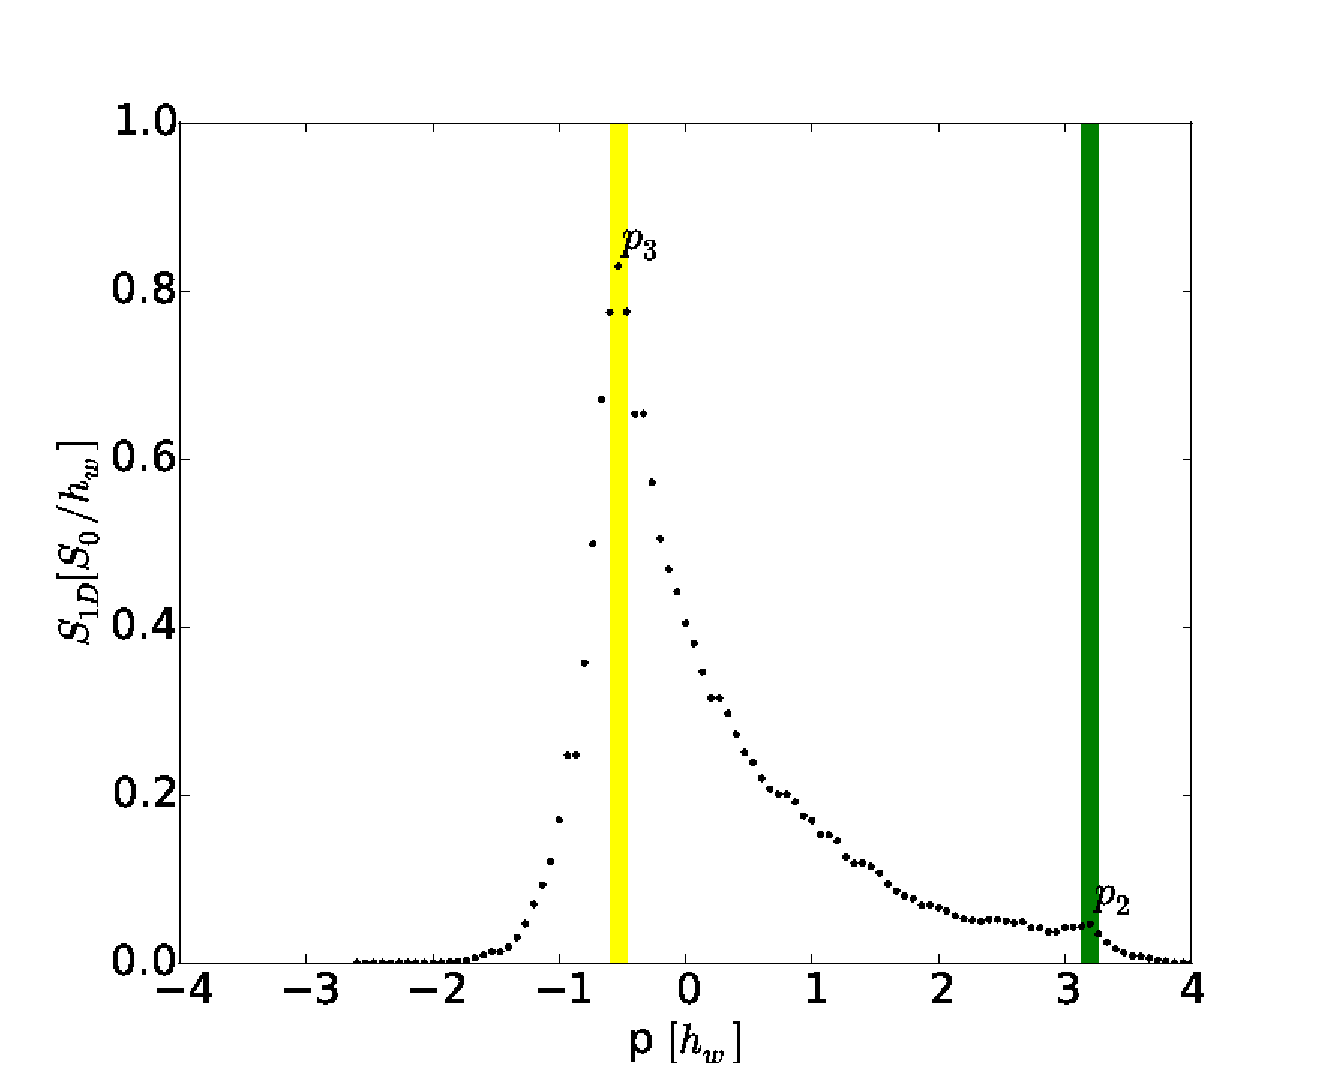
\includegraphics[width = 0.48\textwidth]{figures/M87_shape.eps}
        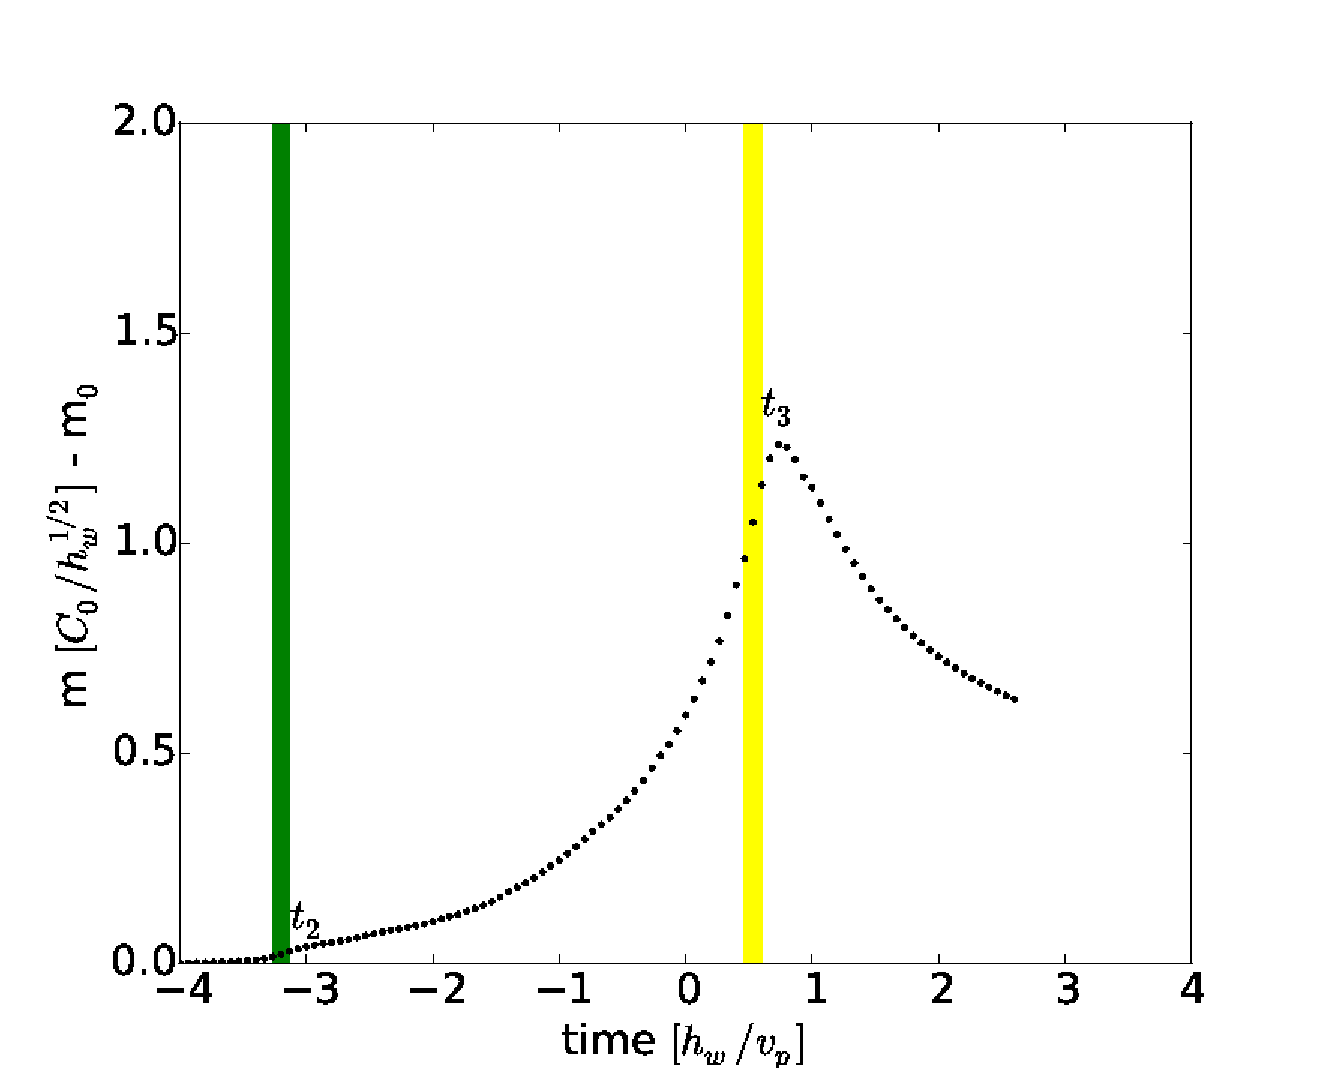
\includegraphics[width = 0.48\textwidth]{figures/M87_lc.eps}
\caption{\label{fig:M87_plots} The one dimensional profile obtained
  from the numerical integration along the ordonata axis of a
  simulated source image is presented in the upper panel. The source
  image was presented in Dexter et al (2012) in the top right-most
  panel of Figure~5 (of the respective paper) as a result of the
  simulations presented in McKinney \& Blandford (2009). The
  corresponding lightcurve associated to the 1D profile is presented
  in the lower panel. The points $\rm p_2$ and $\rm p_3$ mark the
  start and end of the equivalent dark disk and are associated with
  the moments of their overlap with the caustic: $t_2$ and $t_3$;
  $h_{w}$ denotes the maximum width of the crescent.}
\end{figure}


\subsection{Microlensing a simulated image of M87}

\cite{2012MNRAS.421.1517D} have created a radiative image of M87 based on the GRMHD simulations presented in \citep{2009MNRAS.394L.126M}. 
The top right-most image in figure 5 of \cite{2012MNRAS.421.1517D} has been projected to a 1D profile associated to the perpendicular 
direction to a fold caustic approaching the image from the right. The projection is presented in the upper panel of Figure \ref{fig:M87_plots}. 
The amplification values of the flux of light corresponding to a 
microlensing event are presented in the lower panel of Figure \ref{fig:M87_plots}. 
In general, the behaviour of the lightcurve is similar to the geometric crescent source with the caveat that the outer regions 
surrounding the luminous parts of the image have non-zero flux and thus are more extended than the simplified source model.

\section{Fitting mock data}\label{sec:numerics}

Having used the simple model of an ideal fold to gain insight, we now
consider the question of whether the characteristics of a crescent
source could be discerned in real data having noise and systematic
error as well.  Do do so, we first generate a microlensing lightcurve
using a widely-used microlensing code
\citep{1990PhDT.......180W,1999A&A...346L...5W,1999JCoAM.109..353W} to
which we have added a small extension to provide the option of
crescent sources.  We then fit model or template lightcurves ---which
are generated with varied source and other parameters--- to the mock
lightcurve.  The basic technique is the same as in previous studies
\citep[e.g.,][]{2010ApJ...712..658P} though the details are different.

\begin{figure}
\centering
  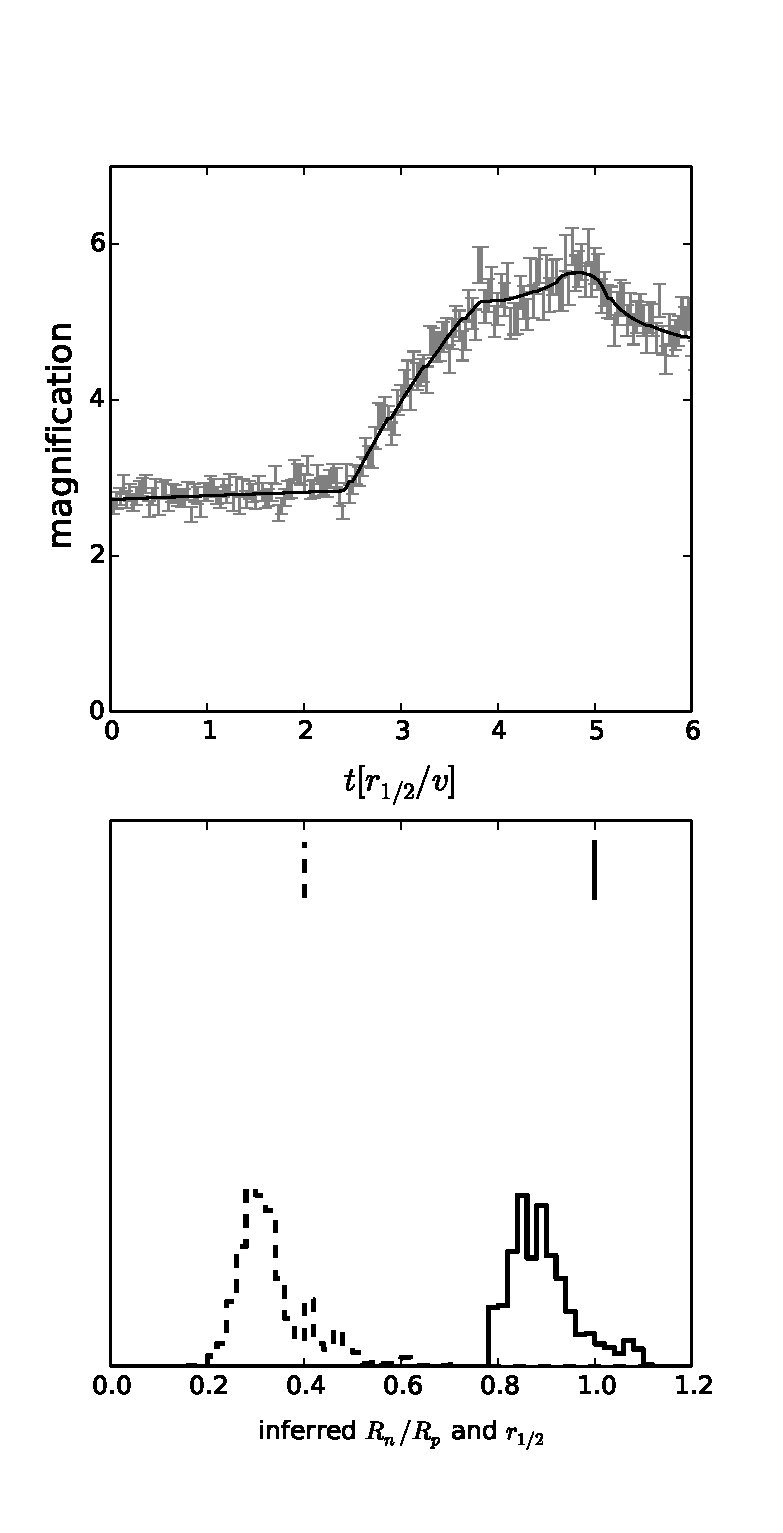
\includegraphics[width=0.5\textwidth]{figures/cc_forward.eps}
\caption{\label{fig:cc_forward} Mock lightcurve fitted with the
  correct source type and caustic.  The upper panel shows the mock
  data points, and running through them is a seven-parameter best fit:
  these being the crescent parameters $(R_p,R_n,a,b)$ and additionally
  the start and end times and the overall normalisation.  (Ideal
  lightcurves for the same crescent parameters appear above in
  Figures~\ref{fig:lightcurve_gauss}, \ref{fig:a_var},
  \ref{fig:lightcurve_crescent} and \ref{fig:char_points}.)  The curve
  has $\chi^2_{(244)}=243, P=0.32$ indicating a good fit.  (The
  subscript 244 refers to degrees of freedom: 251~points less
  7~parameters.)  The lower panel shows the posterior distributions
  for $r_{1/2}$ (solid histogram) and $R_n/R_p$ (dashed histogram).
  Vertical dashes mark the correct values.}
\end{figure}

\begin{figure}
\centering
  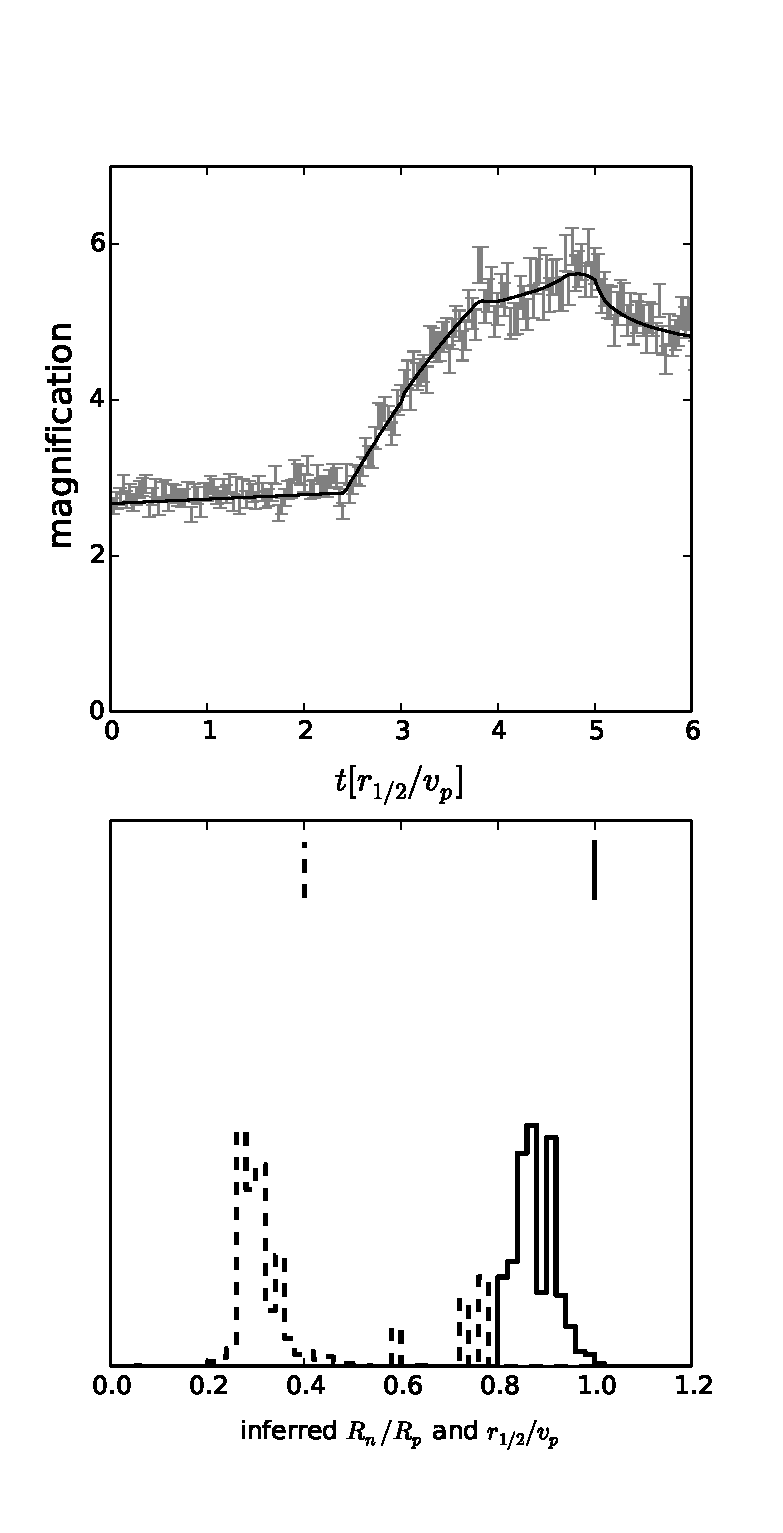
\includegraphics[width=0.5\textwidth]{figures/cc_backward.eps}
\caption{\label{fig:cc_backward} Like Figure~\ref{fig:cc_forward},
  except that the fit is derived from a slightly different caustic
  than the one used to generate the mock data.  The curve has
  $\chi^2_{(244)}=284, P=0.01$ indicating a marginally acceptable
  fit.}
\end{figure}

\begin{figure}
\centering
  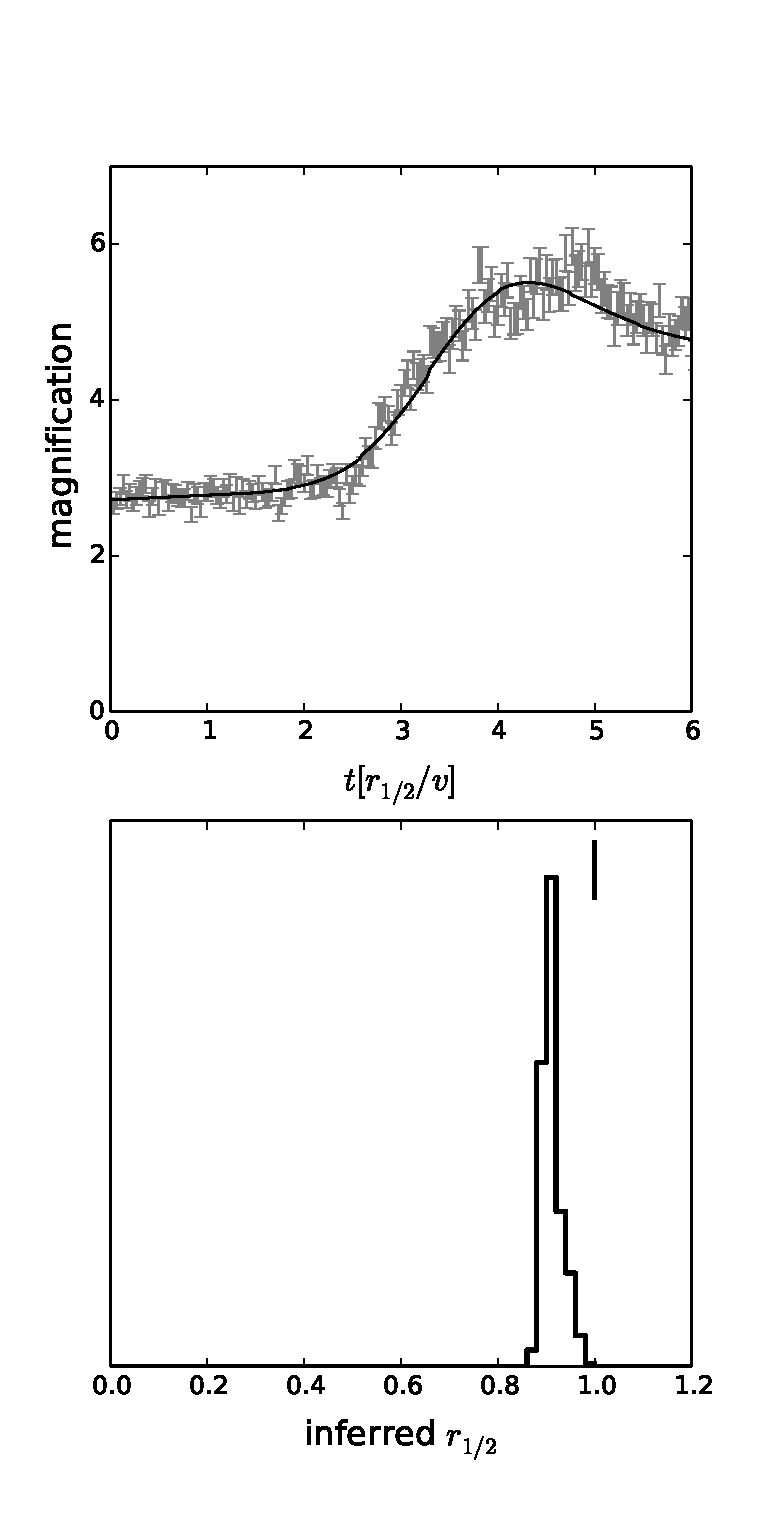
\includegraphics[width=0.5\textwidth]{figures/gc_forward.eps}
\caption{\label{fig:gc_forward} Like Figures~\ref{fig:cc_forward} and
  \ref{fig:cc_backward}, but showing the best fit to a Gaussian
  source.  The histogram shows the posterior distribution of $r_{1/2}$
  (there is no $R_n$).  It appears to show $r_{1/2}$ as accurately
  recovered, but is not to be trusted, because the fit has
  $\chi^2_{(247)}=344, P=3\times10^{-6}$ indicating rejection of the
  Gaussian source.  Looking closely, the curve is a little too shallow
  near $t=3$, and it is unable to fit the second sub-peak near $t=5$.}
\end{figure}

\subsection{Numerical microlensing lightcurves}

The microlensing code uses a ray-shooting technique to compute the
gravitational lensing effect of a mass distribution consisting of
(a)~a smooth component and (b)~a random distribution of point masses
representing stars.  The ray shooting maps a grid of $\vec\theta$ to
$\vec\beta$ using the lens equation (\ref{eqn:lens}).  That is, the
rays are shot from the observer back to the source.  For the
computation of the individual deflection angles
$\vec\alpha(\vec\theta)$ a hierarchical or tree method is used.  The
positions of all lensing masses are put into a grid of $\vec\theta$.
Each grid cell is subdivided into four smaller squares recursively
until every cell contains only one mass.  Nearby masses are added
individually while distance masses are clumped into larger grid cells
whose net contribution is approximated by its first few multipole
moments.  Scaled units are used, with the constant pre-factor in the
deflection angle (\ref{eqn:alpha}) separated out.  The result of ray
shooting is a pixel map on the $\vec\beta$ plane of the number of
lightrays which arrive at the source plane from a particular observer.
This intermediate result is effectively a magnification map on the
source plane.

When generating the magnification map depicted in
Figure~\ref{fig:magnification_map}, which is used in our analysis
below, only two point masses were included.  This was done in order to
have clean fold caustics.  There was no smooth component.

Once the map is created, the lightcurve can be obtained by specifying
the transit path of the source across the map.  The source is moved
along the transit line, one pixel at a time, and at each step the
brightness distribution of the source is convolved
(equation~\ref{eqn:ft2d}) with the magnification map to give the
observable total brightness.  In real life, not only are both lens and
source moving but the lens configuration, and with it the
magnification pattern, is also changing with time.  The first subtlety
is taken care of by a coordinate transformation in this analysis; the
second one is not considered, and the lens configuration is assumed to
be constant in time.

For the purpose of this analysis, it is desirable to mimic the
analytical behaviour of a simple fold as much as possible.
Accordingly, we generated a mock lightcurve by taking a crescent
source along the path CB in Figure~\ref{fig:magnification_map}.  The
crescent parameters (as defined in \S\ref{subsec:crescent}) were
\begin{equation}
   \left(R_p, \frac{R_n}{R_p}, \frac{a}{R_p}, \frac{b}{R_p}\right) =
   (1.31, 0.4, 0, 0.3)
\label{eqn:cp}
\end{equation}
corresponding to $r_{1/2}=1$.  Unit length has 30 pixels on the
magnification map.  The source was carried for 250 pixels along the
path CB, giving 251 brightness values.  Gaussian noise at 4\% of the
current brightness was then added to give the mock data.

The time unit for the light curve is taken to be $r_{1/2}/v_p$
where $v_p$ is the velocity transverse to the caustic.  If we
assume the brightness measurements are nightly, and
$v_p=\rm200\,km/s$, the length of the microlensing event (250
days) is comparable to typical observed events \cite[see
  e.g.,][]{2015ApJ...814L..26M}. The implied $r_{1/2}$ is
$\sim10^{14}\rm\,cm$, which is at the lower end of values inferred for
microlensed X-ray sources, whereas for optical sources, the inferred
$r_{1/2}$ is one to two order of magnitude larger \citep[see, e.g.,
  Figure~8 of][]{0004-637X-769-1-53}.  

The mock data appear in Figures
\ref{fig:cc_forward}--\ref{fig:gc_forward}.  The example values
above for $r_{1/2}$, $v_p$ and the observing frequency are not
important.  What is important is that the observations have enough
sampling and signal-to-noise that the characteristic features of a
crescent source (see e.g., Figure~\ref{fig:char_points}) are not
washed out.


\subsection{Model-fitting results}

We now proceed to fit the mock lightcurve.  MCMC is used to fit source
parameters and additional nuisance parameters (see below) jointly, and
then marginalise out all uninteresting parameters, leaving posterior
distributions for any chosen parameter.

In addition to the source parameters, the fitting procedure includes
three nuisance parameters, namely the brightness normalisation and the
start and end points on the path.  The latter two are equivalent to
considering the location of the caustic with respect to the starting
point and the velocity component of the source transverse to the
caustic (that is, $v_p$).  The orientation of the source track is
another nuisance parameter, but we do not include it, because for a
pure fold, changing the orientation of the source track is equivalent
to changing $v_p$ and the orientation of the source (see
Figure~\ref{fig:infinite_fold}), all parameters that are included.
Since the caustic is not a perfect fold, disregarding the orientation
of the source track can be expected to introduce some systematic
error.

Figures \ref{fig:cc_forward}--\ref{fig:gc_forward} show the numerical
results.  Each of these figures shows the mock data (the same in all
three cases) along with best fits and the fitted values and
uncertainties on $r_{1/2}$ and (if applicable) $R_n/R_p$.

Figure \ref{fig:cc_forward} shows a test of the fitting procedure.
The computer compares the mock data to different template
lightcurves. The templates come from taking a crescent source along
the path CB in Figure~\ref{fig:magnification_map}, but with varied
crescent parameters and varied start and finish points.  As the figure
shows, the lightcurve can be fitted to within the noise, and the
parameters $r_{1/2}$ and $R_n/R_p$ can be recovered.

Figure \ref{fig:cc_backward} attempts a somewhat more realistic
situation.  The mock lightcurve is the same as before, but the
templates come from taking a crescent source along the path AB in
Figure~\ref{fig:magnification_map}.  That is, the mock data and the
templates come from crossings of different caustics.  This mimics the
unavoidable systematic error of not knowing the caustic exactly.  The
fit is slightly degraded, but still acceptable.  The parameters
$r_{1/2}$ and $R_n/R_p$ are still recovered.  The parameters $a/R_p$
and $b/R_p$ were not correctly recovered, which is understandable from
the track change.

Figure \ref{fig:gc_forward} shows the result of attempting to fit
templates from a Gaussian source to the same mock data.  There is a
small but statistically very significant misfit because a Gaussian
source cannot reproduce the part of the lightcurve with the slight
flattening and then a second sub-peak
(cf.~Figure~\ref{fig:char_points}) as the dark part of the crescent
crosses the caustic.  A hint of such a feature is present in recent
caustic-crossing observations of the well-known system Q2237+0305
\citep[see Figure~3 in][]{2015ApJ...814L..26M} though interpretation
as a crescent source is speculation at present.

\section{Discussion}\label{sec:discussion}

In the current paper, we simulate and study the resulting microlensing lightcurves of geometric crescent-shaped sources 
and compare them with the microlensing lightcurves of other simple mathematically describable source profiles. 
In order to mimic the behaviour of the flux of light from the source in the proximity of a fold caustic, 
we make use of the simple approximation described in equation (5). 
The equation would exhaustively describe the magnification map and offer a good universal approximation for the 
particular microlensing regime that we consider. 
Namely, the shape of the caustic boundary in the proximity of the source in the respective plane can be approximated by
 a line due to reason that the local radius of curvature of caustic is orders of magnitude greater than the half-light
 radius of the studied source. 
%In particular cases in which the previously mentioned approximation loses its validity, the impact on the quality of the 
%lightcurves is not evenly distributed. The shape of the lightcurve will be maintained. 
%The data points corresponding to the source position before and during the overlapping of the caustic will be affected by
% smaller errors than the data points corresponding to later times. \\

The first two source profiles that we consider are the uniform disk and the symmetric Gaussian source. 
Both of them can be described by a half-light radius ($r_{1/2}$) and a total unlensed light flux ($S_0$). 
With the two parameters constrained the one-dimensional profiles, as well as the lightcurves of the 
two source, are completely determined, since no free parameter remains. 

The previous statement does not hold for a crescent source.
In the case of the crescent source there are in total five parameters: the integrated flux of the source $S_0$,
 the radii of the bright and dark disks and the displacement of the centers of the two disks on the axes perpendicular and parallel to the caustic. 

%Two of the parameters can be reduced by expressing the results in 
%terms of $S_0$ and $r_{1/2}$. 
%The later being determinable for any set of parameters 
%$R_p, R_n$ and $a^2+b^2$. Moreover, one of the displacement 
%parameters $b$ has no impact on the one-dimensional profile 
%of the source that results from the projection of the source
% image on an axis perpendicular to the caustic. 

Since the one-dimensional source profile that corresponds to an 
axis perpendicular to the caustic contains exhaustively all the 
information regarding the source that can be revealed by the lightcurve, 
the value of the crescent's disks centers displacement parallel to the caustic 
does not have an effect on the shape of the lightcurve. 

Nevertheless, the respective displacement is relevant for the calculation of
of the half-light radius.  Its qualitative effect is to 
decrease the value of the
half-light radius when the absolute value of the parameter is
increased.  In contrast to the simpler source shapes discussed before the
crescent has two additional relevant parameters: the radius of the dark 
disk ($R_n$) and the center displacement in the direction
 perpendicular to the caustic $a$.

Figure \ref{fig:lightcurve_gauss} reveals that the lightcurve of a crescent source has more
visible features than the other two light-curves corresponding to the
disc and Gaussian shape. The parameters $R_n$ and $a$ have strong
influences on the shape of the microlensed lightcurve as can be seen
in Figures~\ref{fig:a_var}, \ref{fig:lightcurve_crescent_back} and
\ref{fig:lightcurve_crescent}.  Moreover, the one-dimensional
source profile corresponding to the direction perpendicular to the
caustic reveal four characteristic points. The overlap of each of
these points with the caustic leaves visible features on the
lightcurve at the corresponding instances of time. In time order,
the instances correspond to the start of the overlap between the
caustic and the bright disk, the start of the overlap between the
caustic and the dark disk, the end of the overlap between the caustic
and dark disk and finally the end of the overlap between the caustic
and the bright disk.

With the different source profiles and their corresponding lightcurves 
studied we can change our point of view of the system to that of an observer. 
The observer would basically detect only the lightcurve of such a source.
 As described in section 4.3 the timing of the onset and 
offset of the previously 
described periods can be used to estimate the values of the radii 
and one of the displacement parameters when assuming a geometric crescent. 
All quantities can be estimated in terms of the relative velocity 
of the source in a direction perpendicular to the caustic.


Furthermore, a simulated image of M87 presented in
\cite{2012MNRAS.421.1517D} has been microlensed
(Figure~\ref{fig:M87_plots}).  On the resulting lightcurve the
instances corresponding to the start and end of the black hole shadow
and caustic overlap were distinguishable.
    
In the case of a high-quality lightcurve, the parameters of a crescent
source can be estimated by simply identifying signatures on the
lightcurve corresponding to transits of the particular source features
across the caustic.  This simple idea can be supplemented with
statistics.  We do so in Section~\ref{sec:numerics}, where we take a
realistic magnification map generated by the microlensing code
from \cite{1999A&A...346L...5W}, compute a caustic-crossing lightcurve
from it, and then fit the lightcurve with other caustic-crossing
templates.  The conclusion is that a crescent source can be
distinguised from a circular source, on the basis of caustic-crossing
lightcurves, if the caustic is a clean but not ideal fold.

The previously mentioned abstract parameters can be related to
physical quantities specific to the central region of a quasar.  As
such the luminous region would correspond to the bright accretion disc
that surrounds the black hole. The later's gravity would cause a
shadow in the bright region limited by the extent of the event horizon
of the black hole. Therefore, the radius of the bright disk would
provide an estimate of the size of the accretion disk and the radius
of the dark disc would provide and estimate of the gravitationally
magnified Schwarzschild radius of the black hole $R_{S}^{magnified} =
\Delta t_{dark} \cdot v_p$.  By $R_{S}^{magnified}$ we refer to the
apparent Schwarzschild radius which is larger than the real value at
large distances due to the black hole's own gravity.  Moreover, the
gravitationally magnified value of the Schwarzschild radius is a
monotonic function of the black hole's mass. Therefore, it can be used
to estimate the mass of the black hole if it was not rotating. In the
previous expression, the $\Delta t_{dark}$ denotes the period of
overlap between the black hole shadow and fold caustic, while $v_p$
denotes the component of the relative velocity of the source and fold
which is perpendicular to the caustic.  The respective velocity is an
unknown, though it can be constrained on a case by case basis to an
order of magnitude or even better. This would require the study of the
dynamics of the stellar structure which contains the gravitational
lens and the bulk transverse velocity of the galaxy with respect to
the observer.  A better estimate of the relative velocity would
facilitate a better estimate of the effective non-rotating black hole
mass associated with the black hole shadow.

    
The parameters whose values cannot be determined due to the 
loss of information from the directions parallel to the 
caustic could be obtained in the eventuality in which 
the same source crosses multiple caustics that are not parallel. 
Multiple crossing of caustics can reveal details of 
the one-dimensional flux profile corresponding to multiple distinct 
directions which would allow the reconstruction of the 
two-dimensional profile analogous to the process through 
which an image of a CT scan is obtained.  

\textit{Author contributions}\\
Prasenjit Saha provided the original idea and plan for the research project as well as multiple contributions to the analysis 
and manuscript preparation. Mihai Tomozeiu simulated and studied the ideal behaviour of the microlensing lightcurves for the 
different source profiles discussed and prepared the manuscript.
Joachim Wambsganss contributed to the research planning and provided the numerical code used by Manuel Rabold to create 
the magnification map and corresponding lightcurves used in the MCMC analysis performed by Irshad Mohammed in the last 
part of the presented work. Both Manuel Rabold and Irshad Mohammed had large contributions in writing the ``Fitting Mock Data'' section.

\section{Acknowledgement}
IM is supported by Fermi Research Alliance, LLC under Contract No. De-AC02-07CH11359 with the United States Department of Energy.
J.W. would like to acknowledge and thank the Pauli Center for Theoretical Studies of ETH Zurich and University of Zurich for 
generous support during the Schr\"odinger visiting professorship in 2013.

\bibliographystyle{mn2e}

\def\apj{ApJ}
\def\apjl{ApJL}
\def\aj{AJ}
\def\mnras{MNRAS}
\def\aap{A\&A}
\def\nat{Nature}
\def\araa{ARAA}
\def\pasa{PASA}
\bibliography{heap}

\end{document}
